% Options for packages loaded elsewhere
\PassOptionsToPackage{unicode}{hyperref}
\PassOptionsToPackage{hyphens}{url}
%
\documentclass[
  11pt,
  english,
  ,doc,floatsintext]{apa6}
\usepackage{lmodern}
\usepackage{setspace}
\usepackage{amssymb,amsmath}
\usepackage{ifxetex,ifluatex}
\ifnum 0\ifxetex 1\fi\ifluatex 1\fi=0 % if pdftex
  \usepackage[T1]{fontenc}
  \usepackage[utf8]{inputenc}
  \usepackage{textcomp} % provide euro and other symbols
\else % if luatex or xetex
  \usepackage{unicode-math}
  \defaultfontfeatures{Scale=MatchLowercase}
  \defaultfontfeatures[\rmfamily]{Ligatures=TeX,Scale=1}
\fi
% Use upquote if available, for straight quotes in verbatim environments
\IfFileExists{upquote.sty}{\usepackage{upquote}}{}
\IfFileExists{microtype.sty}{% use microtype if available
  \usepackage[]{microtype}
  \UseMicrotypeSet[protrusion]{basicmath} % disable protrusion for tt fonts
}{}
\makeatletter
\@ifundefined{KOMAClassName}{% if non-KOMA class
  \IfFileExists{parskip.sty}{%
    \usepackage{parskip}
  }{% else
    \setlength{\parindent}{0pt}
    \setlength{\parskip}{6pt plus 2pt minus 1pt}}
}{% if KOMA class
  \KOMAoptions{parskip=half}}
\makeatother
\usepackage{xcolor}
\IfFileExists{xurl.sty}{\usepackage{xurl}}{} % add URL line breaks if available
\IfFileExists{bookmark.sty}{\usepackage{bookmark}}{\usepackage{hyperref}}
\hypersetup{
  pdftitle={Supplementary materials to `High spatial frequency information in primes hastens happy faces categorization in autistic adults.'},
  pdfauthor={Adeline Lacroix1, Ladislas Nalborczyk2,3, Frédéric Dutheil4, Klara Kovarski5,6, Sylvie Chokron5,6, Marta Garrido7,8, Marie Gomot9, \& Martial Mermillod1},
  pdflang={en-EN},
  hidelinks,
  pdfcreator={LaTeX via pandoc}}
\urlstyle{same} % disable monospaced font for URLs
\usepackage{color}
\usepackage{fancyvrb}
\newcommand{\VerbBar}{|}
\newcommand{\VERB}{\Verb[commandchars=\\\{\}]}
\DefineVerbatimEnvironment{Highlighting}{Verbatim}{commandchars=\\\{\}}
% Add ',fontsize=\small' for more characters per line
\newenvironment{Shaded}{}{}
\newcommand{\AlertTok}[1]{\textcolor[rgb]{1.00,0.00,0.00}{\textbf{#1}}}
\newcommand{\AnnotationTok}[1]{\textcolor[rgb]{0.38,0.63,0.69}{\textbf{\textit{#1}}}}
\newcommand{\AttributeTok}[1]{\textcolor[rgb]{0.49,0.56,0.16}{#1}}
\newcommand{\BaseNTok}[1]{\textcolor[rgb]{0.25,0.63,0.44}{#1}}
\newcommand{\BuiltInTok}[1]{#1}
\newcommand{\CharTok}[1]{\textcolor[rgb]{0.25,0.44,0.63}{#1}}
\newcommand{\CommentTok}[1]{\textcolor[rgb]{0.38,0.63,0.69}{\textit{#1}}}
\newcommand{\CommentVarTok}[1]{\textcolor[rgb]{0.38,0.63,0.69}{\textbf{\textit{#1}}}}
\newcommand{\ConstantTok}[1]{\textcolor[rgb]{0.53,0.00,0.00}{#1}}
\newcommand{\ControlFlowTok}[1]{\textcolor[rgb]{0.00,0.44,0.13}{\textbf{#1}}}
\newcommand{\DataTypeTok}[1]{\textcolor[rgb]{0.56,0.13,0.00}{#1}}
\newcommand{\DecValTok}[1]{\textcolor[rgb]{0.25,0.63,0.44}{#1}}
\newcommand{\DocumentationTok}[1]{\textcolor[rgb]{0.73,0.13,0.13}{\textit{#1}}}
\newcommand{\ErrorTok}[1]{\textcolor[rgb]{1.00,0.00,0.00}{\textbf{#1}}}
\newcommand{\ExtensionTok}[1]{#1}
\newcommand{\FloatTok}[1]{\textcolor[rgb]{0.25,0.63,0.44}{#1}}
\newcommand{\FunctionTok}[1]{\textcolor[rgb]{0.02,0.16,0.49}{#1}}
\newcommand{\ImportTok}[1]{#1}
\newcommand{\InformationTok}[1]{\textcolor[rgb]{0.38,0.63,0.69}{\textbf{\textit{#1}}}}
\newcommand{\KeywordTok}[1]{\textcolor[rgb]{0.00,0.44,0.13}{\textbf{#1}}}
\newcommand{\NormalTok}[1]{#1}
\newcommand{\OperatorTok}[1]{\textcolor[rgb]{0.40,0.40,0.40}{#1}}
\newcommand{\OtherTok}[1]{\textcolor[rgb]{0.00,0.44,0.13}{#1}}
\newcommand{\PreprocessorTok}[1]{\textcolor[rgb]{0.74,0.48,0.00}{#1}}
\newcommand{\RegionMarkerTok}[1]{#1}
\newcommand{\SpecialCharTok}[1]{\textcolor[rgb]{0.25,0.44,0.63}{#1}}
\newcommand{\SpecialStringTok}[1]{\textcolor[rgb]{0.73,0.40,0.53}{#1}}
\newcommand{\StringTok}[1]{\textcolor[rgb]{0.25,0.44,0.63}{#1}}
\newcommand{\VariableTok}[1]{\textcolor[rgb]{0.10,0.09,0.49}{#1}}
\newcommand{\VerbatimStringTok}[1]{\textcolor[rgb]{0.25,0.44,0.63}{#1}}
\newcommand{\WarningTok}[1]{\textcolor[rgb]{0.38,0.63,0.69}{\textbf{\textit{#1}}}}
\usepackage{graphicx,grffile}
\makeatletter
\def\maxwidth{\ifdim\Gin@nat@width>\linewidth\linewidth\else\Gin@nat@width\fi}
\def\maxheight{\ifdim\Gin@nat@height>\textheight\textheight\else\Gin@nat@height\fi}
\makeatother
% Scale images if necessary, so that they will not overflow the page
% margins by default, and it is still possible to overwrite the defaults
% using explicit options in \includegraphics[width, height, ...]{}
\setkeys{Gin}{width=\maxwidth,height=\maxheight,keepaspectratio}
% Set default figure placement to htbp
\makeatletter
\def\fps@figure{htbp}
\makeatother
\setlength{\emergencystretch}{3em} % prevent overfull lines
\providecommand{\tightlist}{%
  \setlength{\itemsep}{0pt}\setlength{\parskip}{0pt}}
\setcounter{secnumdepth}{5}
% Make \paragraph and \subparagraph free-standing
\ifx\paragraph\undefined\else
  \let\oldparagraph\paragraph
  \renewcommand{\paragraph}[1]{\oldparagraph{#1}\mbox{}}
\fi
\ifx\subparagraph\undefined\else
  \let\oldsubparagraph\subparagraph
  \renewcommand{\subparagraph}[1]{\oldsubparagraph{#1}\mbox{}}
\fi
% Manuscript styling
\usepackage{upgreek}
\captionsetup{font=singlespacing,justification=justified}

% Table formatting
\usepackage{longtable}
\usepackage{lscape}
% \usepackage[counterclockwise]{rotating}   % Landscape page setup for large tables
\usepackage{multirow}		% Table styling
\usepackage{tabularx}		% Control Column width
\usepackage[flushleft]{threeparttable}	% Allows for three part tables with a specified notes section
\usepackage{threeparttablex}            % Lets threeparttable work with longtable

% Create new environments so endfloat can handle them
% \newenvironment{ltable}
%   {\begin{landscape}\begin{center}\begin{threeparttable}}
%   {\end{threeparttable}\end{center}\end{landscape}}
\newenvironment{lltable}{\begin{landscape}\begin{center}\begin{ThreePartTable}}{\end{ThreePartTable}\end{center}\end{landscape}}

% Enables adjusting longtable caption width to table width
% Solution found at http://golatex.de/longtable-mit-caption-so-breit-wie-die-tabelle-t15767.html
\makeatletter
\newcommand\LastLTentrywidth{1em}
\newlength\longtablewidth
\setlength{\longtablewidth}{1in}
\newcommand{\getlongtablewidth}{\begingroup \ifcsname LT@\roman{LT@tables}\endcsname \global\longtablewidth=0pt \renewcommand{\LT@entry}[2]{\global\advance\longtablewidth by ##2\relax\gdef\LastLTentrywidth{##2}}\@nameuse{LT@\roman{LT@tables}} \fi \endgroup}

% \setlength{\parindent}{0.5in}
% \setlength{\parskip}{0pt plus 0pt minus 0pt}

% Overwrite redefinition of paragraph and subparagraph by the default LaTeX template
% See https://github.com/crsh/papaja/issues/292
\makeatletter
\renewcommand{\paragraph}{\@startsection{paragraph}{4}{\parindent}%
  {0\baselineskip \@plus 0.2ex \@minus 0.2ex}%
  {-1em}%
  {\normalfont\normalsize\bfseries\itshape\typesectitle}}

\renewcommand{\subparagraph}[1]{\@startsection{subparagraph}{5}{1em}%
  {0\baselineskip \@plus 0.2ex \@minus 0.2ex}%
  {-\z@\relax}%
  {\normalfont\normalsize\itshape\hspace{\parindent}{#1}\textit{\addperi}}{\relax}}
\makeatother

% \usepackage{etoolbox}
\makeatletter
\patchcmd{\HyOrg@maketitle}
  {\section{\normalfont\normalsize\abstractname}}
  {\section*{\normalfont\normalsize\abstractname}}
  {}{\typeout{Failed to patch abstract.}}
\patchcmd{\HyOrg@maketitle}
  {\section{\protect\normalfont{\@title}}}
  {\section*{\protect\normalfont{\@title}}}
  {}{\typeout{Failed to patch title.}}
\makeatother
\shorttitle{Supplementary Materials}
\usepackage{csquotes}
\usepackage{float}
\ifxetex
  % Load polyglossia as late as possible: uses bidi with RTL langages (e.g. Hebrew, Arabic)
  \usepackage{polyglossia}
  \setmainlanguage[]{english}
\else
  \usepackage[shorthands=off,main=english]{babel}
\fi

\title{Supplementary materials to `High spatial frequency information in primes hastens happy faces categorization in autistic adults.'}
\author{Adeline Lacroix\textsuperscript{1}, Ladislas Nalborczyk\textsuperscript{2,3}, Frédéric Dutheil\textsuperscript{4}, Klara Kovarski\textsuperscript{5,6}, Sylvie Chokron\textsuperscript{5,6}, Marta Garrido\textsuperscript{7,8}, Marie Gomot\textsuperscript{9}, \& Martial Mermillod\textsuperscript{1}}
\date{}


\authornote{

Correspondence concerning this article should be addressed to Adeline Lacroix, Laboratoire de Psychologie et NeuroCognition, Univ. Grenoble Alpes, 1251 avenue centrale, Grenoble, France. E-mail: \href{mailto:adeline.lacroix@univ-grenoble-alpes.fr}{\nolinkurl{adeline.lacroix@univ-grenoble-alpes.fr}}

}

\affiliation{\vspace{0.5cm}\textsuperscript{1} LPNC, Univ. Grenoble Alpes, Univ. Savoie Mont Blanc, CNRS, 38000, Grenoble, France\\\textsuperscript{2} Aix Marseille Univ, CNRS, LPC, Marseille, France.\\\textsuperscript{3} Aix Marseille Univ, CNRS, LNC, Marseille, France.\\\textsuperscript{4} Université Clermont Auvergne, CNRS, LaPSCo, CHU Clermont-Ferrand, WittyFit, F-63000 Clermont-Ferrand, France\\\textsuperscript{5} Hôpital Fondation Ophtalmologique A. de Rothschild, Paris, France.\\\textsuperscript{6} Université de Paris, INCC UMR 8002, CNRS, F-75006 Paris, France.\\\textsuperscript{7} Cognitive Neuroscience and Computational Psychiatry Lab, Melbourne School of Psychological Sciences, The University of Melbourne, Australia.\\\textsuperscript{8} Australian Research Council Centre of Excellence for Integrative Brain Function, Australia.\\\textsuperscript{9} UMR 1253 iBrain, Université de Tours, Inserm, Tours, France.}

\begin{document}
\maketitle

{
\setcounter{tocdepth}{3}
\tableofcontents
}
\setstretch{1.25}
\newpage

Parts 1, 2 and 3 of this document correspond to planned analyses (e.g., table of results, complementary analyses without outliers). Parts 4, 5 and 6 correspond to exploratory analyses with Drift Diffusion Models. All the procedure used for these analyses is detailed and can be used as a tutorial.

\hypertarget{model-comparison-for-the-response-time-analysis}{%
\section{Model comparison for the response time analysis}\label{model-comparison-for-the-response-time-analysis}}

\hypertarget{inclusion-of-different-predictors}{%
\subsection{Inclusion of different predictors}\label{inclusion-of-different-predictors}}

We first compared the three following models of increasing complexity and we kept the best one (i.e., the model with the lowest LOOIC - Leave-one-out cross validation information criterion - and the highest weight):

\begin{itemize}
\item
  BMgcp : RT \textasciitilde{} 1 + GroupC * PrimeC * CongC + (1 + CongC * PrimeC \textbar\textbar{} ID) + (1 +
  GroupC * PrimeC * CongC \textbar\textbar{} Target)
\item
  BMgcpe : RT \textasciitilde{} 1 + GroupC * PrimeC * CongC * EmoC + (1 + CongC * PrimeC \emph{
  EmoC \textbar\textbar{} ID) + (1 + GroupC } PrimeC * CongC * EmoC \textbar\textbar{} Target)
\item
  BMgcpes : RT \textasciitilde{} 1 + GroupC * PrimeC * CongC * EmoC * SexC + (1 + CongC * PrimeC * EmoC \textbar\textbar{} ID) + (1 + GroupC * PrimeC * CongC * EmoC * SexC \textbar\textbar{} Target)
\item
  BMgcpesP : RT \textasciitilde{} 1 + GroupC * CongC * PrimeC * EmoC + SexC + SexC:GroupC + (1 + CongC * PrimeC * EmoC \textbar\textbar{} ID) + (1 + GroupC * CongC * PrimeC *EmoC + SexC + SexC:GroupC\textbar\textbar{} Target)
\end{itemize}

\begin{table}[htb]

\begin{center}
\begin{threeparttable}

\caption{\label{tab:modelComp1RT}Expected log pointise predictive density (ELPD) and LOOIC for each BLMM on RT.}

\tiny{

\begin{tabular}{cccccccccc}
\toprule
model & \multicolumn{1}{c}{elpd\_diff} & \multicolumn{1}{c}{se\_diff} & \multicolumn{1}{c}{elpd\_loo} & \multicolumn{1}{c}{se\_elpd\_loo} & \multicolumn{1}{c}{p\_loo} & \multicolumn{1}{c}{se\_p\_loo} & \multicolumn{1}{c}{looic} & \multicolumn{1}{c}{se\_looic} & \multicolumn{1}{c}{Model\_Weights}\\
\midrule
BMgcpe & 0.000 & 0.000 & -92,727.743 & 122.793 & 282.308 & 8.677 & 185,455.485 & 245.587 & 0.745\\
BMgcpesP & -1.408 & 0.755 & -92,729.151 & 122.819 & 288.954 & 8.851 & 185,458.301 & 245.638 & 0.182\\
BMgcpes & -2.323 & 4.451 & -92,730.066 & 123.017 & 326.123 & 9.920 & 185,460.131 & 246.034 & 0.073\\
BMgcp & -180.740 & 21.709 & -92,908.483 & 122.026 & 160.269 & 5.267 & 185,816.965 & 244.051 & 0.000\\
\bottomrule
\end{tabular}

}

\end{threeparttable}
\end{center}

\end{table}

As reported on \emph{Table \ref{tab:modelComp1RT}}, \texttt{BMgcpe} appeared to be the best model compared with models without emotion or with sex (full model or parsimonious model). Hence, we kept this model and then added covariates to this model.

\hypertarget{model-with-covariates}{%
\subsection{Model with covariates}\label{model-with-covariates}}

As preregistered, we added some covariates in the model and again, we kept the best one after model comparison. We included either PIQ or FSIQ and AQ as our two groups differed on these variables.

We compared the following models:

\begin{itemize}
\item
  BMgcpe : RT \textasciitilde{} 1 + GroupC * PrimeC * CongC * EmoC + (1 + CongC * PrimeC \emph{
  EmoC \textbar\textbar{} ID) + (1 + GroupC } PrimeC * CongC * EmoC \textbar\textbar{} Target)
\item
  BMf : RT \textasciitilde{} 1 + GroupC * CongC * PrimeC * EmoC + FSIQc + (1 + CongC * PrimeC * EmoC \textbar\textbar{} ID) + (1 + GroupC * CongC * PrimeC * EmoC \textbar\textbar{} Target)
\item
  BMa : RT \textasciitilde{} 1 + GroupC * CongC * PrimeC * EmoC + AQc + (1 + CongC * PrimeC * EmoC \textbar\textbar{} ID) + (1 + GroupC * CongC * PrimeC *EmoC \textbar\textbar{} Target)
\item
  BMp : RT \textasciitilde{} 1 + GroupC * CongC * PrimeC * EmoC + PIQc + (1 + CongC * PrimeC * EmoC \textbar\textbar{} ID) + (1 + GroupC * CongC * PrimeC *EmoC \textbar\textbar{} Target)
\item
  BMfa : RT \textasciitilde{} 1 + GroupC * CongC * PrimeC * EmoC + FSIQc + AQc + (1 + CongC * PrimeC * EmoC \textbar\textbar{} ID) + (1 + GroupC * CongC * PrimeC *EmoC \textbar\textbar{} Target)
\item
  BMpa : RT \textasciitilde{} 1 + GroupC * CongC * PrimeC * EmoC + PIQc + AQc + (1 + CongC * PrimeC * EmoC \textbar\textbar{} ID) + (1 + GroupC * CongC * PrimeC *EmoC \textbar\textbar{} Target)
\end{itemize}

\begin{table}[htb]

\begin{center}
\begin{threeparttable}

\caption{\label{tab:modelComp2RT}Expected log pointise predictive density (ELPD) and LOOIC for each of the four BLMMs on RT, with covariates}

\tiny{

\begin{tabular}{cccccccccc}
\toprule
model & \multicolumn{1}{c}{elpd\_diff} & \multicolumn{1}{c}{se\_diff} & \multicolumn{1}{c}{elpd\_loo} & \multicolumn{1}{c}{se\_elpd\_loo} & \multicolumn{1}{c}{p\_loo} & \multicolumn{1}{c}{se\_p\_loo} & \multicolumn{1}{c}{looic} & \multicolumn{1}{c}{se\_looic} & \multicolumn{1}{c}{Model\_Weights}\\
\midrule
BMgcpe & 0.000 & 0.000 & -92,727.743 & 122.793 & 282.308 & 8.677 & 185,455.485 & 245.587 & 0.292\\
BMpa & -0.048 & 0.276 & -92,727.790 & 122.794 & 282.289 & 8.639 & 185,455.581 & 245.588 & 0.278\\
BMf & -0.593 & 0.349 & -92,728.336 & 122.817 & 282.583 & 8.698 & 185,456.672 & 245.633 & 0.161\\
BMa & -0.838 & 0.266 & -92,728.581 & 122.796 & 282.747 & 8.681 & 185,457.161 & 245.591 & 0.126\\
BMfa & -1.321 & 0.315 & -92,729.064 & 122.822 & 282.406 & 8.677 & 185,458.128 & 245.643 & 0.078\\
BMp & -1.521 & 0.313 & -92,729.264 & 122.829 & 283.963 & 8.754 & 185,458.528 & 245.657 & 0.064\\
\bottomrule
\end{tabular}

}

\end{threeparttable}
\end{center}

\end{table}

The model without any covariates appeared to be the best model (see \emph{Table \ref{tab:modelComp2RT}}), despite the model with AQ and PIQ seems to be almost equally good. The outcome of these two models are very similar and we kept the more parsimonious (note that there is no evidence of an effect of AQ and PIQ on our data when looking at the output of the model with covariates).

\hypertarget{posterior-predictive-check}{%
\subsection{Posterior predictive check}\label{posterior-predictive-check}}

One way of evaluating the model is to evaluate its predictions. If the model is a good description of the (true) process that generated the observed data, then it should be able to generate data that looks like the observed data. The process of generating data from the estimated posterior distribution is called \emph{posterior predictive checking} and can be used in many different ways using the \texttt{pp\_check()} method (Gabry, Simpson, Vehtari, Betancourt, \& Gelman, \protect\hyperlink{ref-gabry_visualization_2019}{2019}). In \emph{Figure \ref{fig:ppcheckBMgcpe}}, we depict the distribution of the raw data (dark cuurve) along with the distribution of one hundred simulated datasets drawn from the posterior predictive distribution (light thin curves).Our model seems quite good at generating data that fit with our observed data.

\begin{figure}[htb]

{\centering \includegraphics[width=\textwidth]{supplementary_materials_files/figure-latex/ppcheckBMgcpe-1} 

}

\caption{Posterior predictive checking for the BLMM.}\label{fig:ppcheckBMgcpe}
\end{figure}

\newpage

\hypertarget{results}{%
\subsection{Results}\label{results}}

\begin{table}[!h]

\begin{center}
\begin{threeparttable}

\caption{\label{tab:summaryBMgcpe}Estimates and BF01 from the BLMM on RT.}

\small{

\begin{tabular}{ccccccc}
\toprule
Predictors & \multicolumn{1}{c}{Estimate} & \multicolumn{1}{c}{SE} & \multicolumn{1}{c}{Lower} & \multicolumn{1}{c}{Upper} & \multicolumn{1}{c}{Rhat} & \multicolumn{1}{c}{BF01}\\
\midrule
Intercept & 696.93 & 13.69 & 670.39 & 724.09 & 1.00 & NA\\
Group & 66.78 & 24.40 & 16.93 & 113.38 & 1.00 & 0.069\\
Prime & -12.91 & 2.97 & -18.70 & -6.93 & 1.00 & 1.277 x 10\textasciicircum{}-4\\
Congruency & -14.78 & 2.88 & -20.64 & -9.17 & 1.00 & 1.481 x 10\textasciicircum{}-4\\
Emotion & 18.90 & 6.73 & 5.59 & 31.99 & 1.00 & 0.194\\
Group x Prime & -1.30 & 5.84 & -12.74 & 10.12 & 1.00 & 8.487\\
Group x Congruency & -2.42 & 5.43 & -13.10 & 8.15 & 1.00 & 8.386\\
Prime x Congruency & 4.53 & 4.54 & -4.36 & 13.56 & 1.00 & 6.479\\
Group x Emotion & -8.04 & 9.48 & -26.65 & 10.53 & 1.00 & 3.732\\
Prime x Emotion & 3.70 & 4.59 & -5.32 & 12.66 & 1.00 & 8.184\\
Congruency x Emotion & -4.13 & 4.60 & -13.22 & 4.80 & 1.00 & 7.517\\
Group x Prime x Congruency & 2.28 & 8.63 & -14.63 & 19.04 & 1.00 & 5.494\\
Group x Prime x Emotion & 21.19 & 9.23 & 3.08 & 39.21 & 1.00 & 0.403\\
Group x Congruency x Emotion & 6.08 & 9.11 & -11.87 & 23.76 & 1.00 & 4.594\\
Prime x Congruency x Emotion & -8.07 & 9.15 & -26.34 & 9.98 & 1.00 & 3.671\\
Group x Prime x Congruency x Emotion & 7.98 & 17.00 & -25.18 & 41.78 & 1.00 & 2.666\\
\bottomrule
\addlinespace
\end{tabular}

}

\begin{tablenotes}[para]
\normalsize{\textit{Note.} For each predictor, the first two columns represent the estimated
    most probable value for the slope and its standard error (SE). The 'Lower' and 'Upper' are the bounds of the 95\% CrI, whereas the 'Rhat' column reports the Gelman-Rubin statistic regarding the convergence. The last column reports the Bayes factor in favour of the null hypothesis (BF01).}
\end{tablenotes}

\end{threeparttable}
\end{center}

\end{table}

The results of this BLMM are summarized in \emph{Table \ref{tab:summaryBMgcpe}} and are described in the paper.

\newpage

\hypertarget{analysis-without-outliers}{%
\section{Analysis without outliers}\label{analysis-without-outliers}}

We also ran our model removing participants who were outliers (results below Quartile 1 -- 1.5 * Interquartile range or above Quartile 3 + 1.5 * Interquartile Range) on at least half of the condition for accuracy or for RT (3 ASD - 2 females, 1 male - and 3 TD - 2 females, 1 male, as preregistered on \url{https://osf.io/345jv}.

All relevant statistics regarding groups description are set out in \emph{Table \ref{tab:demoWO}}.

\hypertarget{demographical-data}{%
\subsection{Demographical data}\label{demographical-data}}

\begin{table}[htb]

\begin{center}
\begin{threeparttable}

\caption{\label{tab:demoWO}Subject demographics – Means (M), standard deviations (SD) and BF01.}

\begin{tabular}{cccc}
\toprule
 & \multicolumn{1}{c}{Group: ASD (N = 24)} & \multicolumn{1}{c}{Group: TD (N = 31)} & \multicolumn{1}{c}{BF01}\\
\midrule
Age & 33.08 (8.37) & 31.68 (7.29) & 3.04\\
Education & 14.79 (2.69) & 15.90 (2.75) & 1.445\\
FSIQ & 126.42 (13.92) & 113.84 (15.15) & 0.071\\
VIQ & 128.88 (10.63) & 120.52 (14.71) & 0.394\\
PIQ & 118.08 (13.43) & 104.06 (15.14) & 0.026\\
AQ & 36.17 (7.11) & 15.26 (6.24) & 1.026 x 10\textasciicircum{}-13\\
Reading & 0.10 (0.88) & -0.07 (0.55) & 2.61\\
Stroop Effect & 0.45 (0.81) & 0.55 (0.77) & 3.306\\
\bottomrule
\addlinespace
\end{tabular}

\begin{tablenotes}[para]
\normalsize{\textit{Note.} *FSIQ = Full Scale Intelligence Quotient; VIQ = Verbal Intelligence Quotient; PIQ = Performance Intelligence Quotient ; AQ = Autism-Spectrum Quotient.}
\end{tablenotes}

\end{threeparttable}
\end{center}

\end{table}

\hypertarget{posterior-predictive-check-1}{%
\subsection{Posterior predictive check}\label{posterior-predictive-check-1}}

\begin{figure}[!h]

{\centering 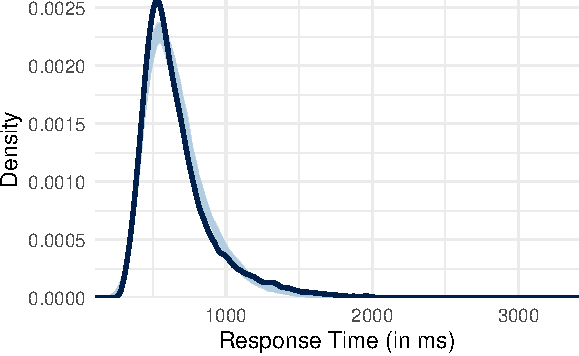
\includegraphics[width=\textwidth]{supplementary_materials_files/figure-latex/ppcheckBMwo-1} 

}

\caption{Posterior predictive checking for the BLMM without outliers.}\label{fig:ppcheckBMwo}
\end{figure}

\newpage

\hypertarget{results-1}{%
\subsection{Results}\label{results-1}}

\begin{table}[!h]

\begin{center}
\begin{threeparttable}

\caption{\label{tab:summaryBMwo}Estimates from the ExGaussian BLMM on RT without outliers.}

\small{

\begin{tabular}{ccccccc}
\toprule
Predictors & \multicolumn{1}{c}{Estimate} & \multicolumn{1}{c}{SE} & \multicolumn{1}{c}{Lower} & \multicolumn{1}{c}{Upper} & \multicolumn{1}{c}{Rhat} & \multicolumn{1}{c}{BF01}\\
\midrule
Intercept & 667.48 & 12.51 & 643.00 & 692.00 & 1.00 & NA\\
Group & 52.29 & 22.12 & 7.77 & 94.71 & 1.00 & 0.16\\
Prime & -11.19 & 2.71 & -16.48 & -5.87 & 1.00 & 0.01\\
Congruency & -11.43 & 2.66 & -16.72 & -6.15 & 1.00 & 0.01\\
Emotion & 18.02 & 5.99 & 6.27 & 29.70 & 1.00 & 0.11\\
Group x Prime & 1.22 & 5.11 & -8.76 & 11.18 & 1.00 & 9.91\\
Group x Congruency & 0.73 & 4.74 & -8.65 & 10.06 & 1.00 & 10.62\\
Prime x Congruency & 6.09 & 4.64 & -3.08 & 15.26 & 1.00 & 4.70\\
Group x Emotion & -11.31 & 8.34 & -27.51 & 5.31 & 1.00 & 2.51\\
Prime x Emotion & 1.02 & 4.47 & -7.77 & 9.85 & 1.00 & 11.74\\
Congruency x Emotion & -0.40 & 4.55 & -9.35 & 8.46 & 1.00 & 11.19\\
Group x Prime x Congruency & 9.28 & 8.79 & -8.12 & 26.42 & 1.00 & 3.33\\
Group x Prime x Emotion & 24.83 & 8.96 & 7.31 & 42.21 & 1.00 & 0.15\\
Group x Congruency x Emotion & 11.32 & 8.84 & -5.88 & 28.78 & 1.00 & 2.63\\
Prime x Congruency x Emotion & -5.08 & 9.30 & -23.30 & 13.47 & 1.00 & 4.80\\
Group x Prime x Congruency x Emotion & 17.19 & 17.56 & -17.54 & 51.71 & 1.00 & 1.86\\
\bottomrule
\end{tabular}

}

\end{threeparttable}
\end{center}

\end{table}

\newpage

\hypertarget{analysis-on-inverse-efficiency-score-ies}{%
\section{Analysis on Inverse Efficiency Score (IES)}\label{analysis-on-inverse-efficiency-score-ies}}

As preregistered, we also fitted models on the IES (= Response Time/Accuracy) to take into account the accuracy.

\hypertarget{inclusion-of-different-predictors-1}{%
\subsection{Inclusion of different predictors}\label{inclusion-of-different-predictors-1}}

We compared the 3 following models:

\begin{itemize}
\item
  IBMgcp : IES \textasciitilde{} 1 + GroupC * CongC * PrimeC + (1 \textbar{} ID)
\item
  IBMgcpe: IES \textasciitilde{} 1 + GroupC * CongC * PrimeC * EmoC+ (1 \textbar{} ID)
\item
  IBMgcpes : IES \textasciitilde{} 1 + GroupC * CongC * PrimeC * EmoC * SexC + (1 \textbar{} ID)
\item
  IBMgcpesP: IES \textasciitilde{} 1 + GroupC * CongC * PrimeC * EmoC + SexC + SexC : EmoC + (1 \textbar{} ID)
\end{itemize}

\begin{table}[htb]

\begin{center}
\begin{threeparttable}

\caption{\label{tab:modelCompIES1}Expected log pointise predictive density (ELPD) and LOOIC for each of the three BLMM on IES.}

\tiny{

\begin{tabular}{cccccccccc}
\toprule
model & \multicolumn{1}{c}{elpd\_diff} & \multicolumn{1}{c}{se\_diff} & \multicolumn{1}{c}{elpd\_loo} & \multicolumn{1}{c}{se\_elpd\_loo} & \multicolumn{1}{c}{p\_loo} & \multicolumn{1}{c}{se\_p\_loo} & \multicolumn{1}{c}{looic} & \multicolumn{1}{c}{se\_looic} & \multicolumn{1}{c}{Model\_Weights}\\
\midrule
IBMgcpe & 0.000 & 0.000 & -2,798.330 & 28.402 & 87.995 & 13.260 & 5,596.661 & 56.805 & 0.535\\
IBMgcpesP & -0.147 & 0.283 & -2,798.478 & 28.456 & 88.162 & 13.335 & 5,596.955 & 56.912 & 0.462\\
IBMgcpes & -5.391 & 3.453 & -2,803.722 & 28.166 & 99.316 & 13.894 & 5,607.443 & 56.332 & 0.002\\
IBMgcp & -11.643 & 6.458 & -2,809.973 & 27.255 & 79.990 & 11.494 & 5,619.946 & 54.510 & 0.000\\
\bottomrule
\end{tabular}

}

\end{threeparttable}
\end{center}

\end{table}

The model \texttt{IBMgcpe} seemed to be the best one (see \emph{Table \ref{tab:modelCompIES1}}).

\hypertarget{inclusion-of-covariates}{%
\subsection{Inclusion of covariates}\label{inclusion-of-covariates}}

We then included covariates in the best model. We compared the following models:\\
- IBMfa : IES \textasciitilde{} 1 + GroupC * CongC * PrimeC * EmoC + FSIQ + AQ + (1 \textbar{} ID)

\begin{itemize}
\item
  IBMf : IES \textasciitilde{} 1 + GroupC * CongC * PrimeC * EmoC + FSIQ +(1 \textbar{} ID)
\item
  IBMa : IES \textasciitilde{} 1 + GroupC * CongC * PrimeC * EmoC + AQ +(1 \textbar{} ID)
\item
  IBMpa : IES \textasciitilde{} 1 + GroupC * CongC * PrimeC * EmoC + PIQ + AQ + (1 \textbar{} ID)
\item
  IBMp : IES \textasciitilde{} 1 + GroupC * CongC * PrimeC * EmoC + PIQ + (1 \textbar{} ID)
\end{itemize}

\begin{table}[htb]

\begin{center}
\begin{threeparttable}

\caption{\label{tab:modelCompIES2}Expected log pointise predictive density (ELPD) and LOOIC for each of the four BLMM on IES, with covariates.}

\tiny{

\begin{tabular}{cccccccccc}
\toprule
model & \multicolumn{1}{c}{elpd\_diff} & \multicolumn{1}{c}{se\_diff} & \multicolumn{1}{c}{elpd\_loo} & \multicolumn{1}{c}{se\_elpd\_loo} & \multicolumn{1}{c}{p\_loo} & \multicolumn{1}{c}{se\_p\_loo} & \multicolumn{1}{c}{looic} & \multicolumn{1}{c}{se\_looic} & \multicolumn{1}{c}{Model\_Weights}\\
\midrule
IBMf & 0.000 & 0.000 & -2,796.274 & 27.783 & 85.749 & 11.867 & 5,592.549 & 55.565 & 0.222\\
IBMa & -1.287 & 0.820 & -2,797.561 & 28.081 & 87.203 & 12.582 & 5,595.122 & 56.161 & 0.196\\
IBMpa & -1.311 & 1.159 & -2,797.586 & 28.189 & 87.227 & 12.787 & 5,595.171 & 56.378 & 0.191\\
IBMp & -1.399 & 1.242 & -2,797.673 & 28.225 & 87.259 & 12.851 & 5,595.346 & 56.451 & 0.175\\
IBMfa & -1.742 & 1.374 & -2,798.016 & 28.362 & 87.495 & 12.993 & 5,596.032 & 56.724 & 0.124\\
IBMgcpe & -2.056 & 1.509 & -2,798.330 & 28.402 & 87.995 & 13.260 & 5,596.661 & 56.805 & 0.091\\
\bottomrule
\end{tabular}

}

\end{threeparttable}
\end{center}

\end{table}

The model \texttt{IBMf}, with FSIQ as a covariate, appear to be the best model (see \emph{Table \ref{tab:modelCompIES2}}). We checked the validity of this model with posterior predictive check (cf.~\emph{Figure 2}), which appeared to be good.

\hypertarget{posterior-predictive-check-2}{%
\subsection{Posterior predictive check}\label{posterior-predictive-check-2}}

\begin{figure}[!h]

{\centering 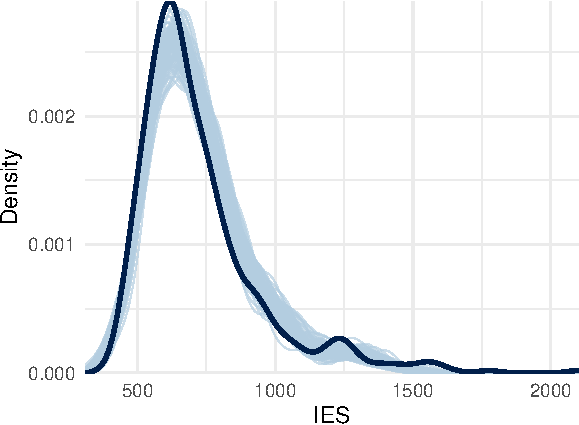
\includegraphics[width=\textwidth]{supplementary_materials_files/figure-latex/ppcheckIBMf-1} 

}

\caption{Posterior predictive checking for BLMM concerning the IES.}\label{fig:ppcheckIBMf}
\end{figure}

\newpage

\hypertarget{results-2}{%
\subsection{Results}\label{results-2}}

\begin{table}[htb]

\begin{center}
\begin{threeparttable}

\caption{\label{tab:summaryIBMf}Estimates from the ExGaussian BLMM concerning the IES.}

\small{

\begin{tabular}{ccccccc}
\toprule
Predictors & \multicolumn{1}{c}{Estimate} & \multicolumn{1}{c}{SE} & \multicolumn{1}{c}{Lower} & \multicolumn{1}{c}{Upper} & \multicolumn{1}{c}{Rhat} & \multicolumn{1}{c}{BF01}\\
\midrule
Intercept & 730.19 & 19.53 & 691.32 & 767.97 & 1.00 & NA\\
Group & 83.46 & 31.59 & 20.32 & 144.61 & 1.00 & 0.061\\
Congruency & -36.86 & 5.55 & -47.93 & -26.20 & 1.00 & 5.523 x 10\textasciicircum{}-17\\
Prime & -16.09 & 5.06 & -26.09 & -6.28 & 1.00 & 0.039\\
Emotion & 20.35 & 5.47 & 9.75 & 31.05 & 1.00 & 0.015\\
FSIQ & -41.42 & 19.11 & -78.60 & -4.36 & 1.00 & 0.255\\
Group x Congruency & 8.64 & 9.92 & -10.97 & 27.83 & 1.00 & 3.475\\
Group x Prime & -6.75 & 9.94 & -26.23 & 12.64 & 1.00 & 3.931\\
Prime x Congruency & 6.30 & 9.64 & -12.76 & 25.07 & 1.00 & 4.156\\
Group x Emotion & -28.79 & 10.71 & -50.09 & -7.95 & 1.00 & 0.123\\
Congruency x Emotion & 1.10 & 9.70 & -17.88 & 20.03 & 1.00 & 5.232\\
Prime x Emotion & 12.70 & 9.66 & -6.34 & 31.78 & 1.00 & 2.202\\
Group x Prime x Congruency & 1.44 & 18.36 & -34.82 & 37.11 & 1.00 & 2.692\\
Group x Congruency x Emotion & 8.27 & 18.48 & -28.12 & 44.56 & 1.00 & 2.446\\
Group x Prime x Emotion & 56.90 & 18.43 & 20.70 & 92.78 & 1.00 & 0.025\\
Prime x Congruency x Emotion & -10.15 & 18.37 & -45.64 & 25.80 & 1.00 & 2.312\\
Group x Prime x Congruency x Emotion & 3.08 & 31.31 & -57.82 & 64.40 & 1.00 & 1.626\\
\bottomrule
\end{tabular}

}

\end{threeparttable}
\end{center}

\end{table}

\newpage

\hypertarget{visual-data-exploration}{%
\section{Visual data exploration}\label{visual-data-exploration}}

\begin{figure}[!htb]

{\centering 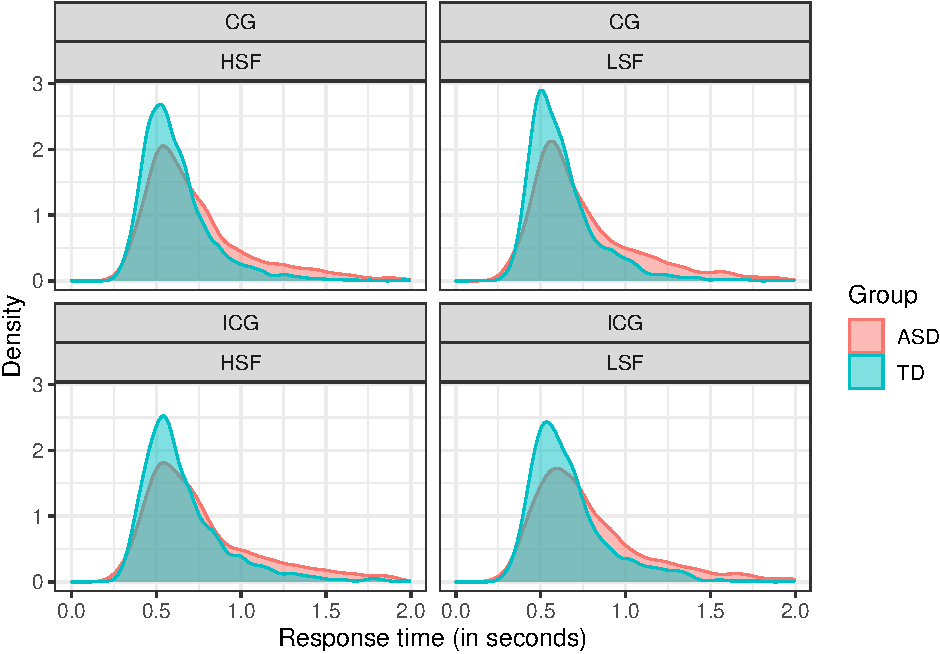
\includegraphics[width=0.75\linewidth]{supplementary_materials_files/figure-latex/data-1} 

}

\caption{Distribution of RTs per Group, Congruency, and Prime.}\label{fig:data}
\end{figure}

Figure \ref{fig:data} shows that the distributions of response times (RTs) are roughly similar across conditions, with slightly slower and more spread RTs in the ASD group as compared to the TD group. In Figure \ref{fig:correctness1}, we plot the distribution of RTs for correct versus incorrect responses according to the characteristics of the participants (Sex and Group). In Figure \ref{fig:correctness2}, we make a similar plot, now faceting by condition (i.e., congruency and prime type).

\begin{figure}[!h]

{\centering 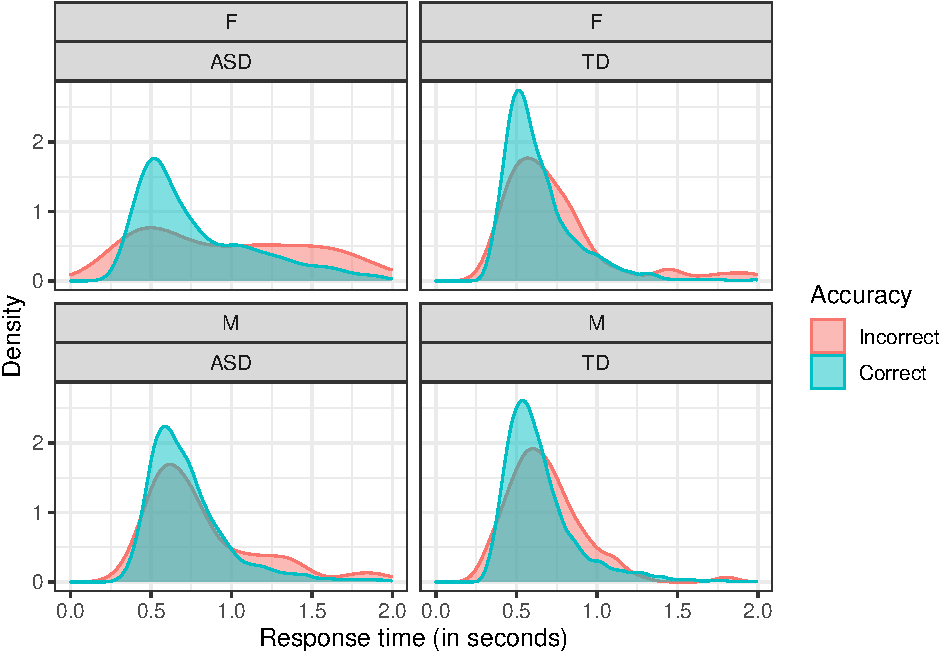
\includegraphics[width=0.75\linewidth]{supplementary_materials_files/figure-latex/correctness1-1} 

}

\caption{Distribution of RTs for correct and incorrect responses according to Sex and Group. Incorrect responses are in pink and correct responses in blue.}\label{fig:correctness1}
\end{figure}

\begin{figure}[!htb]

{\centering 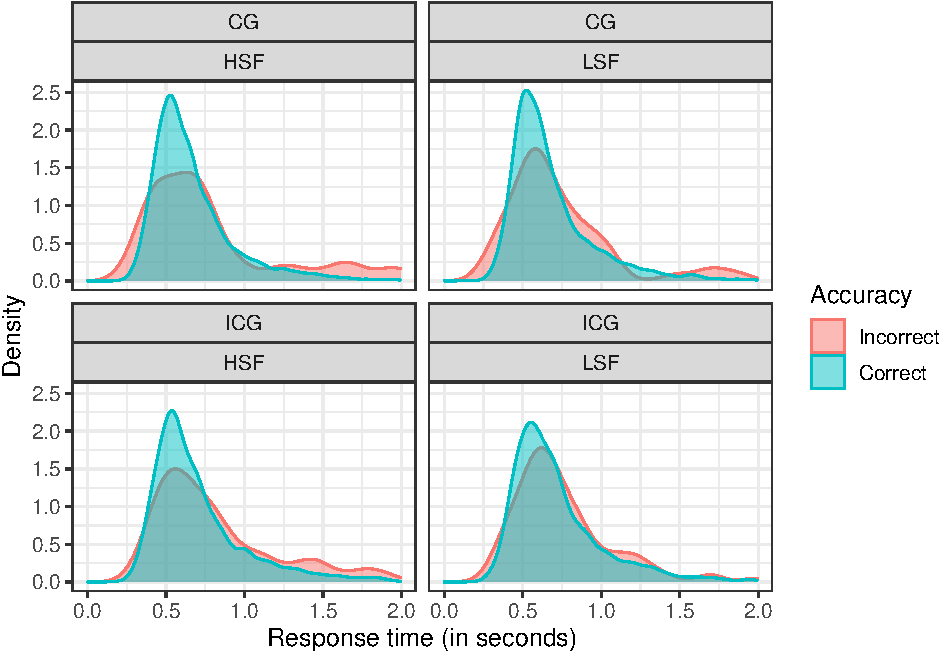
\includegraphics[width=0.75\linewidth]{supplementary_materials_files/figure-latex/correctness2-1} 

}

\caption{Distribution of RTs for correct and incorrect responses according to Congruency and Prime. Incorrect responses are in pink and correct responses in blue.}\label{fig:correctness2}
\end{figure}

\newpage

\hypertarget{diffusion-decision-modelling}{%
\section{Diffusion decision modelling}\label{diffusion-decision-modelling}}

Diffusion decision models (DDM) allow detailed explanations of behaviour in two-alternative forced choice tasks. We know that the data collected in such tasks obey some law-like patterns. For instance, RT distributions are generally positively skewed, with the skewness increasing with task difficulty. We also know that the mean of the RTs is proportional to the standard deviation of the RTs. Increases in the difficulty usually lead to increased RTs and decreased accuracy. Moreover, changes in difficulty also produces regular changes in the distribution of RTs, most notably in its spread but not much in its shape (for a review, see Forstmann, Ratcliff, \& Wagenmakers, \protect\hyperlink{ref-forstmann_sequential_2016}{2016}). Therefore, several models have been proposed to account for the peculiarities of the data coming from such tasks as well as to relate it to the underlying cognitive processes.

\hypertarget{what-is-a-diffusion-decision-model}{%
\subsection{What is a diffusion decision model?}\label{what-is-a-diffusion-decision-model}}

The vanilla (i.e., original) diffusion decision model (the \enquote{Wiener model}) is a continuous-time evidence accumulation model for binary choice tasks (Ratcliff, \protect\hyperlink{ref-ratcliff_theory_1978}{1978}). It assumes that in each trial evidence is accumulated in a noisy (diffusion) process by a single accumulator. As shown in Figure \ref{fig:wiener-figure}, evidence accumulation starts at some point (the starting point or \enquote{bias}) and continues until the accumulator hits one of the two decision bounds in which case the corresponding response is given. The total response time is the sum of the decision time from the accumulation process plus non-decisional components (Vandekerckhove, Verheyen, \& Tuerlinckx, \protect\hyperlink{ref-vandekerckhove_crossed_2010}{2010}; Wabersich \& Vandekerckhove, \protect\hyperlink{ref-wabersich_rwiener_2014}{2014}; Wagenmakers, \protect\hyperlink{ref-wagenmakers_methodological_2009-1}{2009}).\footnote{Where diffusion is to be understood as the continuous equivalent of a random-walk.} In other words, this kind of model provides a \emph{decomposition} of RT data that isolates components (of processing) from stimulus encoding to decision so that they can be studied individually (Ratcliff \& McKoon, \protect\hyperlink{ref-ratcliff_diffusion_2008}{2008}; Wagenmakers, Van Der Maas, \& Grasman, \protect\hyperlink{ref-wagenmakers_ez-diffusion_2007}{2007}).



\begin{figure}[!htb]

{\centering 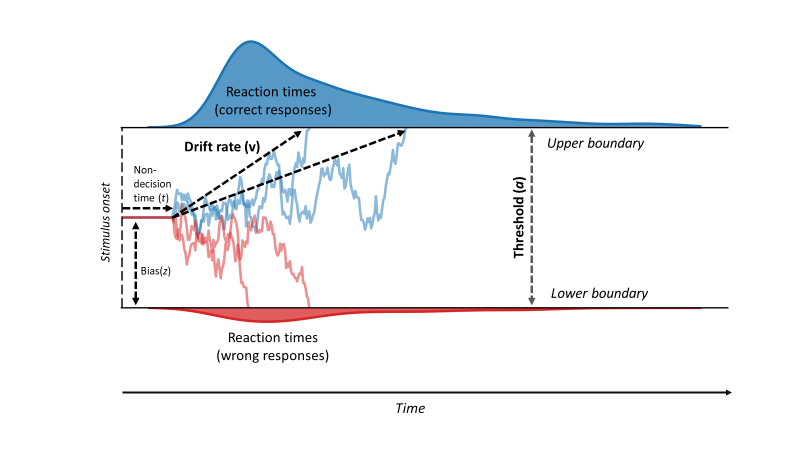
\includegraphics[width=0.75\linewidth]{figures/wiener_figure} 

}

\caption{A graphical illustration of the Wiener diffusion model. Figure from Vinding, Lindeløv, Xiao, Chan, and Sørensen (\protect\hyperlink{ref-vinding_volition_2018}{2018}).}\label{fig:wiener-figure}
\end{figure}

In sum, the original Wiener model allows decomposing responses to a binary choice tasks and corresponding response times into four latent processes (Singmann, \protect\hyperlink{ref-singmann_diffusionux2fwiener_2017}{2017}):

\begin{itemize}
\item
  The \textbf{drift rate} \(\delta\) (delta) is the average slope of the accumulation process towards the boundaries (i.e., it represents the average amount of evidence accumulated per unit time). The larger the (absolute value of the) drift rate, the stronger the evidence for the corresponding response option (thus quantifying the \enquote{ease of processing}).
\item
  The \textbf{boundary separation} \(\alpha\) (alpha) is the distance between the two decision bounds and can be interpreted as a measure of response caution, with high \(\alpha\) meaning high caution.
\item
  The \textbf{starting point} (or bias) \(\beta\) (beta) of the accumulation process is a measure of response bias towards one of the two response boundaries (it is sometimes fixed to \(0.5\) in case of correct vs.~incorrect boundaries, but it need not to be).
\item
  The \textbf{non-decision time} \(\tau\) (tau) captures all non-decisional processes such as stimulus encoding and (motor) response processes.
\end{itemize}

An important decision that has to be made before setting up a model is which parameters are allowed to differ between which conditions. One common constraint of the Wiener model is that the parameters that are set before the evidence accumulation process starts (i.e., boundary separation, starting point, and non-decision time) cannot change based on stimulus characteristics that are not known to the participant before the start of the trial. However, as the response time was recorded from the presentation of the \emph{target}, the participant already had knowledge about the prime when the evidence accumulations began. Thus, the characteristics of the item (i.e., in our case, congruency and spatial characteristics) are only allowed to affect the drift rate, but we compared this model to an augmented model including the nature of the prime (i.e., LSF vs.~HSF) and an interaction with Group on the response bias (starting point). Also note that all stimulus-related variables are manipulated within-subject. Thus, the maximal random-effects structure (Barr, Levy, Scheepers, \& Tily, \protect\hyperlink{ref-barr_random_2013-1}{2013}) entails corresponding random-effects parameters for each fixed-effect. To set up the model we need to invoke the \texttt{brms::brmsformula()} function and construct one formula for each of the four parameters of the Wiener model.

\hypertarget{fitting-the-model}{%
\subsection{Fitting the model}\label{fitting-the-model}}

We fitted all models using the \texttt{brms} package (Bürkner, \protect\hyperlink{ref-R-brms_a}{2017}).

\begin{Shaded}
\begin{Highlighting}[]
\CommentTok{# defining the model formula (one "linear model" per parameter)}
\NormalTok{formula <-}\StringTok{ }\KeywordTok{brmsformula}\NormalTok{(}
  \CommentTok{# drift rate (delta)}
\NormalTok{  RT }\OperatorTok{|}\StringTok{ }\KeywordTok{dec}\NormalTok{(ACC) }\OperatorTok{~}\StringTok{ }\DecValTok{1} \OperatorTok{+}\StringTok{ }\NormalTok{GroupC }\OperatorTok{*}\StringTok{ }\NormalTok{CongC }\OperatorTok{*}\StringTok{ }\NormalTok{PrimeC }\OperatorTok{+}\StringTok{ }\NormalTok{(}\DecValTok{1} \OperatorTok{|}\StringTok{ }\NormalTok{ID) }\OperatorTok{+}\StringTok{ }\NormalTok{(}\DecValTok{1} \OperatorTok{|}\StringTok{ }\NormalTok{Target),}
  \CommentTok{# boundary separation parameter (alpha)}
\NormalTok{  bs }\OperatorTok{~}\StringTok{ }\DecValTok{1} \OperatorTok{+}\StringTok{ }\NormalTok{GroupC }\OperatorTok{+}\StringTok{ }\NormalTok{(}\DecValTok{1} \OperatorTok{|}\StringTok{ }\NormalTok{ID) }\OperatorTok{+}\StringTok{ }\NormalTok{(}\DecValTok{1} \OperatorTok{|}\StringTok{ }\NormalTok{Target),}
  \CommentTok{# non-decision time (tau)}
\NormalTok{  ndt }\OperatorTok{~}\StringTok{ }\DecValTok{1} \OperatorTok{+}\StringTok{ }\NormalTok{GroupC }\OperatorTok{+}\StringTok{ }\NormalTok{(}\DecValTok{1} \OperatorTok{|}\StringTok{ }\NormalTok{ID) }\OperatorTok{+}\StringTok{ }\NormalTok{(}\DecValTok{1} \OperatorTok{|}\StringTok{ }\NormalTok{Target),}
  \CommentTok{# starting point or bias (beta)}
\NormalTok{  bias }\OperatorTok{~}\StringTok{ }\DecValTok{1} \OperatorTok{+}\StringTok{ }\NormalTok{GroupC }\OperatorTok{*}\StringTok{ }\NormalTok{PrimeC }\OperatorTok{+}\StringTok{ }\NormalTok{(}\DecValTok{1} \OperatorTok{|}\StringTok{ }\NormalTok{ID) }\OperatorTok{+}\StringTok{ }\NormalTok{(}\DecValTok{1} \OperatorTok{|}\StringTok{ }\NormalTok{Target)}
\NormalTok{  )}
\CommentTok{# defining the priors}
\NormalTok{priors <-}\StringTok{ }\KeywordTok{c}\NormalTok{(}
  \CommentTok{# priors for the intercepts}
  \KeywordTok{prior}\NormalTok{(}\StringTok{"normal(0, 5)"}\NormalTok{, }\DataTypeTok{class =} \StringTok{"Intercept"}\NormalTok{),}
  \KeywordTok{prior}\NormalTok{(}\StringTok{"normal(0, 1)"}\NormalTok{, }\DataTypeTok{class =} \StringTok{"Intercept"}\NormalTok{, }\DataTypeTok{dpar =} \StringTok{"bs"}\NormalTok{),}
  \KeywordTok{prior}\NormalTok{(}\StringTok{"normal(0, 1)"}\NormalTok{, }\DataTypeTok{class =} \StringTok{"Intercept"}\NormalTok{, }\DataTypeTok{dpar =} \StringTok{"ndt"}\NormalTok{),}
  \KeywordTok{prior}\NormalTok{(}\StringTok{"normal(0, 1)"}\NormalTok{, }\DataTypeTok{class =} \StringTok{"Intercept"}\NormalTok{, }\DataTypeTok{dpar =} \StringTok{"bias"}\NormalTok{),}
  \CommentTok{# priors for the slopes}
  \KeywordTok{prior}\NormalTok{(}\StringTok{"normal(0, 1)"}\NormalTok{, }\DataTypeTok{class =} \StringTok{"b"}\NormalTok{),}
  \CommentTok{# priors on the SD of the varying effects}
  \KeywordTok{prior}\NormalTok{(}\StringTok{"exponential(1)"}\NormalTok{, }\DataTypeTok{class =} \StringTok{"sd"}\NormalTok{)}
\NormalTok{  )}
\end{Highlighting}
\end{Shaded}

We then fit this model below using the \texttt{brms::brm()} function. We run eight chains, each for 5000 iterations and using the first 2000 iterations used as warmup (i.e., the first 2000 samples of each chain are discarded from the final analysis). This results in a total of \(8 \times (5000 - 2000) = 24000\) samples from the (joint) posterior distribution that will be used for inference.

\begin{Shaded}
\begin{Highlighting}[]
\CommentTok{# specify initial values to help the model start sampling}
\CommentTok{# (with small variation between chains)}
\NormalTok{chains <-}\StringTok{ }\DecValTok{8} \CommentTok{# number of chains}
\NormalTok{epsilon <-}\StringTok{ }\FloatTok{0.1} \CommentTok{# variability in starting value for the NDT intercept}
\NormalTok{get_init_value <-}\StringTok{ }\ControlFlowTok{function}\NormalTok{(x) }\KeywordTok{list}\NormalTok{(}\DataTypeTok{Intercept_ndt =} \KeywordTok{rnorm}\NormalTok{(}\DataTypeTok{n =} \DecValTok{1}\NormalTok{, }\DataTypeTok{mean =}\NormalTok{ x, }\DataTypeTok{sd =}\NormalTok{ epsilon) )}
\NormalTok{inits_drift <-}\StringTok{ }\KeywordTok{replicate}\NormalTok{(chains, }\KeywordTok{get_init_value}\NormalTok{(}\OperatorTok{-}\DecValTok{3}\NormalTok{), }\DataTypeTok{simplify =} \OtherTok{FALSE}\NormalTok{)}
\CommentTok{# fitting the model}
\NormalTok{varying_effects_prime <-}\StringTok{ }\KeywordTok{brm}\NormalTok{(}
\NormalTok{  formula, }
  \DataTypeTok{data =}\NormalTok{ df,}
  \CommentTok{# specifying the family and link functions for each parameter}
  \DataTypeTok{family =} \KeywordTok{wiener}\NormalTok{(}
    \DataTypeTok{link =} \StringTok{"identity"}\NormalTok{, }\DataTypeTok{link_bs =} \StringTok{"log"}\NormalTok{,}
    \DataTypeTok{link_ndt =} \StringTok{"log"}\NormalTok{, }\DataTypeTok{link_bias =} \StringTok{"logit"}
\NormalTok{    ),}
  \CommentTok{# comment this line to use default priors}
  \DataTypeTok{prior =}\NormalTok{ priors,}
  \CommentTok{# list of initialisation values}
  \DataTypeTok{inits =}\NormalTok{ inits_drift,}
  \DataTypeTok{init_r =} \FloatTok{0.05}\NormalTok{,}
  \DataTypeTok{warmup =} \DecValTok{2000}\NormalTok{, }\DataTypeTok{iter =} \DecValTok{5000}\NormalTok{,}
  \DataTypeTok{chains =}\NormalTok{ chains, }\DataTypeTok{cores =}\NormalTok{ chains,}
  \DataTypeTok{control =} \KeywordTok{list}\NormalTok{(}\DataTypeTok{adapt_delta =} \FloatTok{0.99}\NormalTok{, }\DataTypeTok{max_treedepth =} \DecValTok{15}\NormalTok{),}
  \CommentTok{# saves the model (as .rds) or loads it if it already exists}
  \DataTypeTok{file =} \StringTok{"models/wiener_varying_effects_prime.rds"}\NormalTok{,}
  \CommentTok{# needed for hypothesis testing}
  \DataTypeTok{sample_prior =} \OtherTok{TRUE}
\NormalTok{  )}
\end{Highlighting}
\end{Shaded}

\hypertarget{ddm-interpretation-of-the-results}{%
\section{DDM: Interpretation of the results}\label{ddm-interpretation-of-the-results}}

\hypertarget{model-comparison}{%
\subsection{Model comparison}\label{model-comparison}}

We first compared the previous model with a similar model including an effect of the prime on the response bias parameter. As response time was recorded from the presentation of the target, it is possible that the prime influenced the response bias toward accurate (or erroneous) responses. Table \ref{tab:model_comparison} reports the expected log-pointwise predictive density (ELPD, a measure of the model's fit), the number of effective parameters (p\_WAIC, a measure of the model's complexity) and the WAIC, as well as the difference of these criteria between the two models.

\begin{table}[htb]

\begin{center}
\begin{threeparttable}

\caption{\label{tab:model_comparison}Expected log-pointwise predictive density (ELPD) and WAIC for the two DDMs.}

\tiny{

\begin{tabular}{cccccccccc}
\toprule
model & \multicolumn{1}{c}{elpd\_diff} & \multicolumn{1}{c}{se\_diff} & \multicolumn{1}{c}{elpd\_waic} & \multicolumn{1}{c}{se\_elpd\_waic} & \multicolumn{1}{c}{p\_waic} & \multicolumn{1}{c}{se\_p\_waic} & \multicolumn{1}{c}{waic} & \multicolumn{1}{c}{se\_waic} & \multicolumn{1}{c}{Model\_Weights}\\
\midrule
varying\_effects\_prime & 0.000 & 0.000 & 4,123.821 & 139.639 & 287.720 & 11.840 & -8,247.641 & 279.279 & 0.878\\
varying\_effects & -16.991 & 6.742 & 4,106.830 & 139.704 & 284.992 & 11.778 & -8,213.659 & 279.409 & 0.122\\
\bottomrule
\end{tabular}

}

\end{threeparttable}
\end{center}

\end{table}

From this table (especially from the last two columns) we see that the varying-effects model including an effect of Prime on the response bias has the lowest WAIC, which can be interpreted by saying that this model is estimated to be the closest to the \enquote{true model} in an information-theoretic sense, or equivalently, that it is expected to have the lowest out-of-sample deviance. In the following, we therefore report estimates from this model.

\hypertarget{interpreting-the-output}{%
\subsection{Interpreting the output}\label{interpreting-the-output}}

Now that we have fitted the model, we are left with the task of interpreting the output from the best model. As can be seen from the model summary displayed below, the output of the model is a (joint) posterior distribution over all parameters of the model. We can marginalise this joint distribution to obtain the (marginal) posterior distribution on each parameter, which is given by the \texttt{summary()} method.

\begin{Shaded}
\begin{Highlighting}[]
\CommentTok{# prints a summary of the model}
\KeywordTok{summary}\NormalTok{(varying_effects_prime)}
\end{Highlighting}
\end{Shaded}

\begin{verbatim}
##  Family: wiener 
##   Links: mu = identity; bs = log; ndt = log; bias = logit 
## Formula: RT | dec(ACC) ~ 1 + GroupC * CongC * PrimeC + (1 | ID) + (1 | Target) 
##          bs ~ 1 + GroupC + (1 | ID) + (1 | Target)
##          ndt ~ 1 + GroupC + (1 | ID) + (1 | Target)
##          bias ~ 1 + GroupC * PrimeC + (1 | ID) + (1 | Target)
##    Data: df (Number of observations: 15685) 
## Samples: 8 chains, each with iter = 5000; warmup = 2000; thin = 1;
##          total post-warmup samples = 24000
## 
## Group-Level Effects: 
## ~ID (Number of levels: 66) 
##                    Estimate Est.Error l-95% CI u-95% CI Rhat Bulk_ESS Tail_ESS
## sd(Intercept)          0.79      0.08     0.66     0.96 1.00     6017    10261
## sd(bs_Intercept)       0.18      0.02     0.15     0.23 1.00     8283    13322
## sd(ndt_Intercept)      0.32      0.03     0.27     0.39 1.00     4905     8658
## sd(bias_Intercept)     0.30      0.04     0.23     0.38 1.00    10921    15016
## 
## ~Target (Number of levels: 30) 
##                    Estimate Est.Error l-95% CI u-95% CI Rhat Bulk_ESS Tail_ESS
## sd(Intercept)          0.18      0.03     0.12     0.24 1.00     8719    14004
## sd(bs_Intercept)       0.01      0.01     0.00     0.03 1.00     5586     8798
## sd(ndt_Intercept)      0.02      0.01     0.01     0.04 1.00     5545     5153
## sd(bias_Intercept)     0.03      0.02     0.00     0.08 1.00     5317     9585
## 
## Population-Level Effects: 
##                     Estimate Est.Error l-95% CI u-95% CI Rhat Bulk_ESS Tail_ESS
## Intercept               3.08      0.11     2.87     3.29 1.00     3748     7299
## bs_Intercept            0.73      0.03     0.68     0.78 1.00     5185     8832
## ndt_Intercept          -1.32      0.04    -1.40    -1.24 1.00     3008     5300
## bias_Intercept         -0.42      0.05    -0.51    -0.33 1.00    10148    15306
## GroupC                 -0.06      0.20    -0.46     0.34 1.00     3317     6734
## CongC                   0.31      0.02     0.27     0.36 1.00    40138    16830
## PrimeC                 -0.10      0.04    -0.18    -0.02 1.00    22252    18876
## GroupC:CongC           -0.11      0.05    -0.20    -0.01 1.00    37221    17639
## GroupC:PrimeC          -0.00      0.08    -0.16     0.15 1.00    21239    18092
## CongC:PrimeC            0.06      0.05    -0.04     0.15 1.00    37475    17664
## GroupC:CongC:PrimeC    -0.02      0.10    -0.21     0.18 1.00    40402    16929
## bs_GroupC               0.05      0.05    -0.05     0.14 1.00     5538     9940
## ndt_GroupC              0.25      0.08     0.08     0.41 1.00     2896     4804
## bias_GroupC             0.06      0.09    -0.12     0.24 1.00    10071    13948
## bias_PrimeC             0.16      0.03     0.11     0.21 1.00    21880    19283
## bias_GroupC:PrimeC      0.01      0.05    -0.10     0.11 1.00    21301    17848
## 
## Samples were drawn using sampling(NUTS). For each parameter, Bulk_ESS
## and Tail_ESS are effective sample size measures, and Rhat is the potential
## scale reduction factor on split chains (at convergence, Rhat = 1).
\end{verbatim}

We can retrieve the samples from the joint posterior distribution using the \texttt{brms::posterior\_samples()} method.

\begin{Shaded}
\begin{Highlighting}[]
\CommentTok{# retrieves posterior samples (for all parameters)}
\NormalTok{varying_effects_prime <-}\StringTok{ }\KeywordTok{readRDS}\NormalTok{(}\DataTypeTok{file =} \StringTok{"models/wiener_varying_effects_prime.rds"}\NormalTok{)}
\NormalTok{post <-}\StringTok{ }\KeywordTok{posterior_samples}\NormalTok{(varying_effects_prime)}
\CommentTok{# the "post" object has 24.000 rows (number of posterior samples) and}
\CommentTok{# 396 columns (number of parameters)}
\KeywordTok{dim}\NormalTok{(post)}
\end{Highlighting}
\end{Shaded}

\begin{verbatim}
## [1] 24000   396
\end{verbatim}

\begin{Shaded}
\begin{Highlighting}[]
\CommentTok{# displaying the first six samples for the first 5 parameters}
\KeywordTok{head}\NormalTok{(post[, }\DecValTok{1}\OperatorTok{:}\DecValTok{5}\NormalTok{])}
\end{Highlighting}
\end{Shaded}

\begin{verbatim}
##   b_Intercept b_bs_Intercept b_ndt_Intercept b_bias_Intercept    b_GroupC
## 1    2.904270      0.6586814       -1.275385       -0.3706857 -0.11342708
## 2    2.972417      0.6528011       -1.308810       -0.4090769  0.03222316
## 3    2.868398      0.6492471       -1.292156       -0.2937770 -0.20980861
## 4    3.050407      0.7175195       -1.257030       -0.3241950 -0.02612217
## 5    3.105057      0.7030418       -1.215820       -0.2389826  0.01180252
## 6    3.122955      0.6999282       -1.217508       -0.2114922 -0.03119975
\end{verbatim}

Which outputs a matrix with parameters of the model in columns and posterior samples in rows. Let's examine these results for each parameter in more details.

\hypertarget{drift-rate}{%
\subsubsection{Drift rate}\label{drift-rate}}

From there, we can study the marginal posterior distribution for each parameter of interest. For instance, Figure \ref{fig:posterior-intercept-drift} represents the posterior distribution of the intercept for the drift rate (i.e., the overall mean value of the drift rate).

\begin{Shaded}
\begin{Highlighting}[]
\CommentTok{# retrieves the posterior samples for the average drift rate}
\NormalTok{average_drift <-}\StringTok{ }\NormalTok{post}\OperatorTok{$}\NormalTok{b_Intercept}
\CommentTok{# plotting it}
\KeywordTok{plotPost}\NormalTok{(}
\NormalTok{  average_drift, }\DataTypeTok{showMode =} \OtherTok{TRUE}\NormalTok{,}
  \DataTypeTok{xlab =} \KeywordTok{expression}\NormalTok{(}\KeywordTok{paste}\NormalTok{(beta[}\DecValTok{0}\NormalTok{][}\KeywordTok{paste}\NormalTok{(}\StringTok{"["}\NormalTok{, delta, }\StringTok{"]"}\NormalTok{)] ) )}
\NormalTok{  )}
\end{Highlighting}
\end{Shaded}

\begin{figure}[!htb]

{\centering 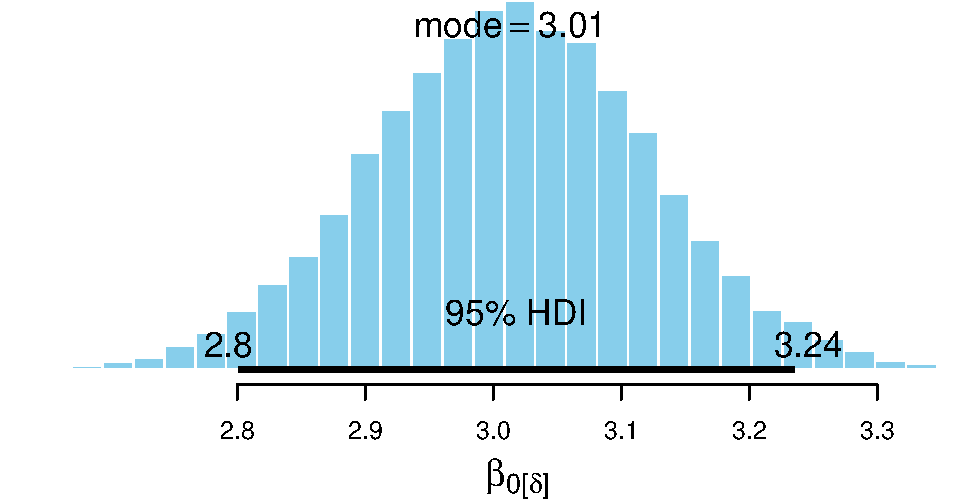
\includegraphics[width=0.75\linewidth]{supplementary_materials_files/figure-latex/posterior-intercept-drift-1} 

}

\caption{Posterior distribution of the intercept for the drift rate. The mode (i.e., the most probable value) and the 95\% credible interval are also displayed.}\label{fig:posterior-intercept-drift}
\end{figure}

Figure \ref{fig:posterior-intercept-drift} reveals (consistently with the summary displayed previously) that the most probable value for the intercept of the drift rate (given our model, the priors, and the data) is 3.014, and that there is a 95\% probability that the population value for this parameter lies in the interval ranging from 2.799 to 3.234. More interestingly, we can inspect the posterior distribution of the slopes for the effects of \texttt{Group}, \texttt{Prime}, and \texttt{Cong}.

\begin{figure}[!htb]

{\centering 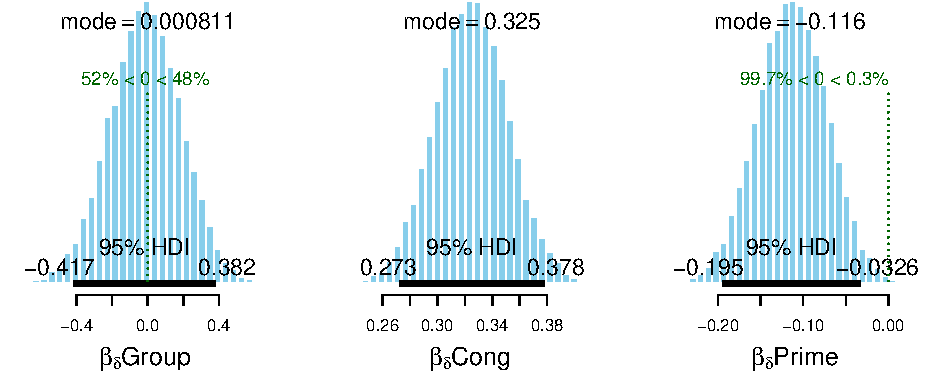
\includegraphics[width=1\linewidth]{supplementary_materials_files/figure-latex/posterior-slopes-drift-1} 

}

\caption{Posterior distribution of the slopes for the drift rate, for Group, Prime, and Cong (respectively). The mode (i.e., the most probable value) and the 95\% credible interval are also displayed.}\label{fig:posterior-slopes-drift}
\end{figure}

Figure \ref{fig:posterior-slopes-drift} reveals that \texttt{Cong} increased the drift rate whereas \texttt{Prime} decreased it (recall that the drift rate can be interpreted as the \enquote{ease of processing}),\footnote{As \texttt{Cong} and \texttt{Prime} were coded using sum contrasts (-0.5 vs.~0.5), these effects can be interpreted as follows: going from incongruent to congruent stimuli or to HSF to LSF stimuli is associated with \enquote{more} ease of processing.} whereas the effect of \texttt{Group} is estimated to be quasi null (cf.~later hypothesis testing). What about interactions?

\begin{figure}[!htb]

{\centering 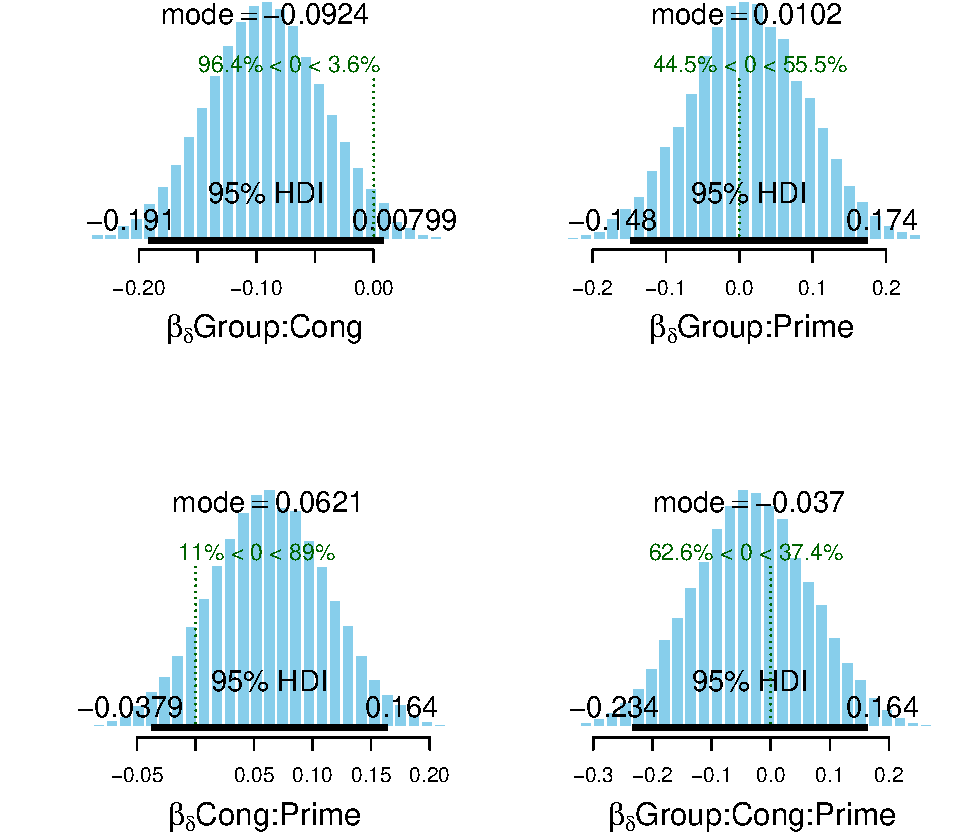
\includegraphics[width=0.75\linewidth]{supplementary_materials_files/figure-latex/posterior-interactions-drift-1} 

}

\caption{Posterior distribution of the interactions slopes for the drift rate. The mode (i.e., the most probable value) and the 95\% credible interval are also displayed.}\label{fig:posterior-interactions-drift}
\end{figure}

Figure \ref{fig:posterior-interactions-drift} reveals that the interaction between \texttt{Group} and \texttt{Prime} and the double interaction between \texttt{Group}, \texttt{Cong}, and \texttt{Prime} were most probably close to zero. However, the interaction between \texttt{Group} and \texttt{Cong} seems reliably negative, which can be interpreted as follows: going from TD to ASD is associated with a decrease in the effect of \texttt{Cong} (which was positive) on the drift rate. In other words, whereas the main effect of \texttt{Cong} indicates that congruent stimuli are easier to process than incongruent stimuli, this interaction indicates that this effect is less pronounced in the ASD group than in the TD group. The interaction between \texttt{Cong} and \texttt{Prime} can be interpreted similarly, where going from incongruent to congruent stimuli increase the effect of \texttt{Prime} (which was positive) on the drift rate (and reciprocally).

\hypertarget{boundary-separation}{%
\subsubsection{Boundary separation}\label{boundary-separation}}

Recall that the boundary separation parameter can be interpreted as a measure of response caution (with high \(\alpha\) corresponding to high response caution), and that the linear model for this parameter is on the log scale (i.e., we used a log link function): \(\log(\alpha_{i}) = \beta_{0} + \beta_{1} \cdot \text{Group}_{i}\).

\begin{figure}[!htb]

{\centering 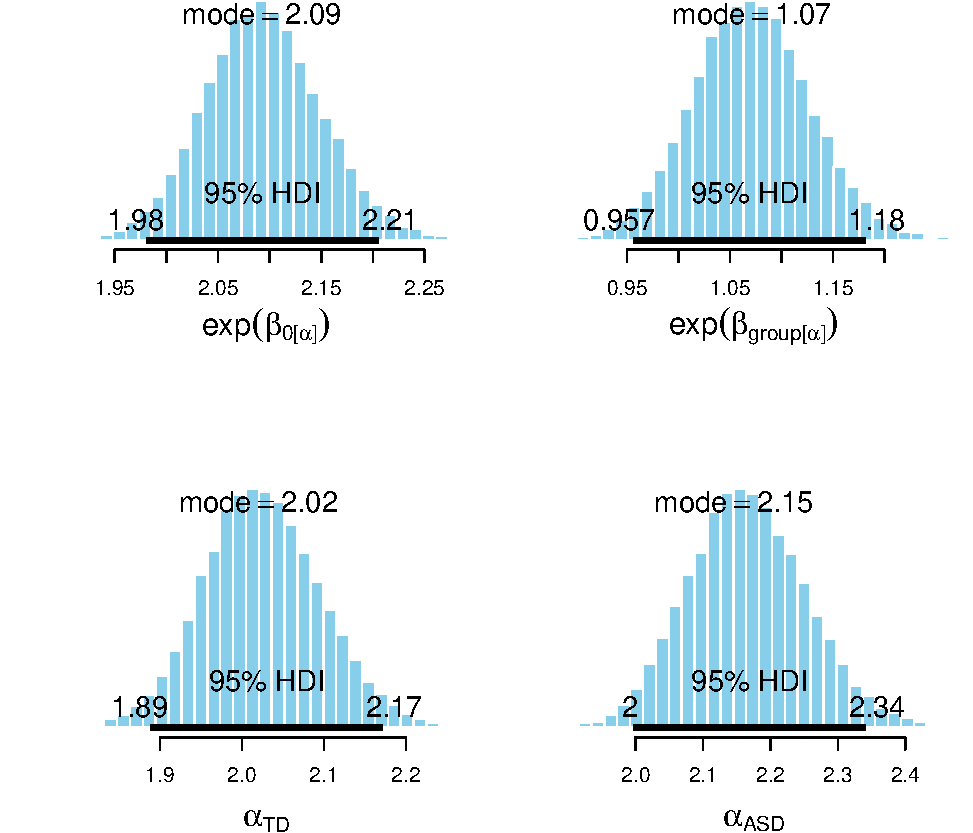
\includegraphics[width=0.75\linewidth]{supplementary_materials_files/figure-latex/posterior-bs-1} 

}

\caption{Posterior distribution of the intercept and the slope for Group for the boundary separation. The upper two distributions are the distributions of the intercept and the slope (on the linear scale). The lower two plots are the posterior distributions of the boundary separation parameter in the TD and ASD groups, respectively (on the linear scale).}\label{fig:posterior-bs}
\end{figure}

Therefore, we have to apply the inverse link function (i.e., \(\exp(\cdot)\)) to the parameter to be able to interpret it. Taking \(\exp(\beta_{1})\) gives the proportional change in the value of the boundary-separation parameter when we go from the TD group to the ASD group (see upper right panel of Figure \ref{fig:posterior-bs}). In our case, \(\exp(\beta_{1}) \approx\) 1.083, which means that going from TD to ASD leads to an increase of approximately 8 \% in the value of the boundary-separation parameter. In other words, response caution seems higher in the ASD group (see lower right panel of Figure \ref{fig:posterior-bs}) than in the TD group (see lower left panel of Figure \ref{fig:posterior-bs}).

\hypertarget{starting-point}{%
\subsubsection{Starting point}\label{starting-point}}

The starting point is a measure of response bias towards one of the two response boundaries (here, correct vs.~incorrect) and is bounded between 0 and 1. The linear model for this parameter is on the logit (log-odds) scale: \(\log(\frac{\beta_{i}}{1 - \beta_{i}}) = \beta_{0} + \beta_{1} \cdot \text{Group}_{i}\). Therefore, we have to apply the inverse link function (i.e., \(\mathrm{logit}^{-1}(\beta_{i}) = \mathrm{logistic}(\beta_{i}) = \frac{1}{1 + \exp(- \beta_{i})} = \frac{\exp(\beta_{i})}{\exp(\beta_{i}) + 1}\)) to the parameter to be able to interpret it on its natural scale (i.e., between 0 and 1).

\begin{figure}[!htb]

{\centering 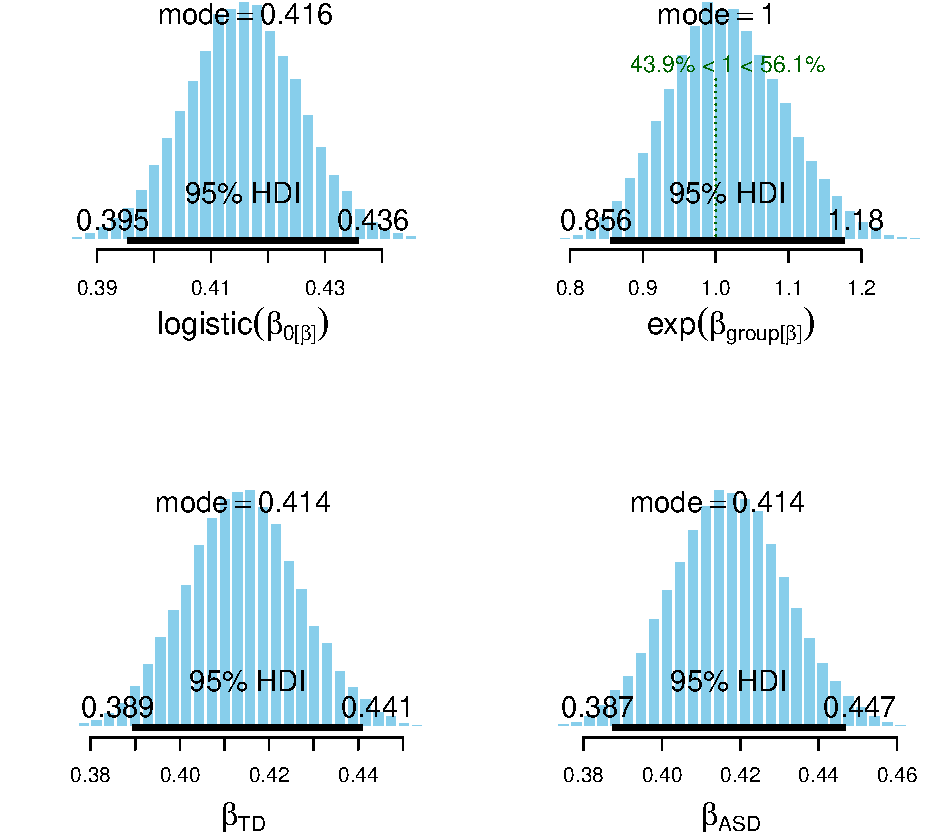
\includegraphics[width=0.75\linewidth]{supplementary_materials_files/figure-latex/posterior-bias-1} 

}

\caption{Posterior distribution of the intercept and the slope for Group for the sarting point (bias). The upper two distributions are the distributions of the intercept (on the natural scale of the parameter) and the exponential of the slope (giving an odds ratio). The lower two plots are the posterior distributions of the estimated statting points in the TD and ASD groups, respectively (on the linear scale).}\label{fig:posterior-bias}
\end{figure}

Taking the exponential of the slope gives an odds ratio of approximately 0.99, which indicates that the odds of producing a correct answer (vs.~an incorrect one) are approximately the same in both groups. This can also be read from the posterior distribution of the bias parameter in the ASD group, when compared with the posterior distribution of the bias parameter in the TD group. We can also plot the posterior distribution of the difference between ASD and TD (cf.~Figure \ref{fig:posterior-bias-difference}).

\begin{figure}[!htb]

{\centering 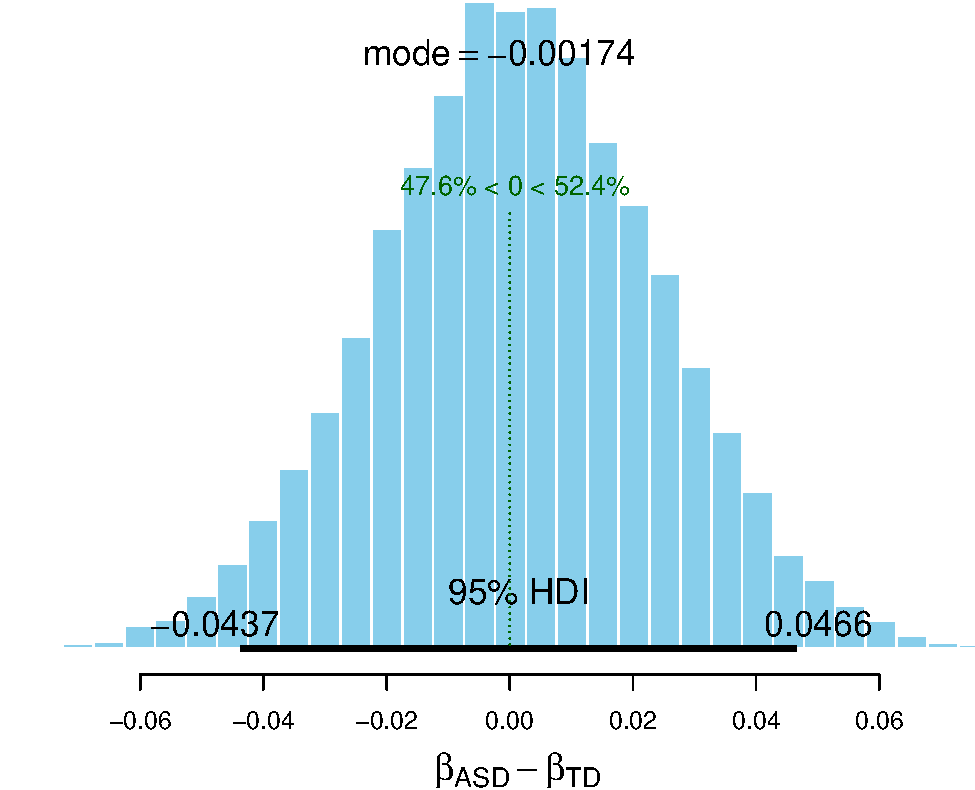
\includegraphics[width=0.5\linewidth]{supplementary_materials_files/figure-latex/posterior-bias-difference-1} 

}

\caption{Posterior distribution of the difference between the estimated starting point in the ASD group and the estimated starting point in the TD group.}\label{fig:posterior-bias-difference}
\end{figure}

As shown in Figure \ref{fig:posterior-bias-prime}, the effect of \texttt{Prime} was positive, which means that HSF (vs.~LSF) primes were associated with a \enquote{bias} towards accurate responses. No interaction effect was found between \texttt{Group} and \texttt{Prime}.

\begin{figure}[!htb]

{\centering 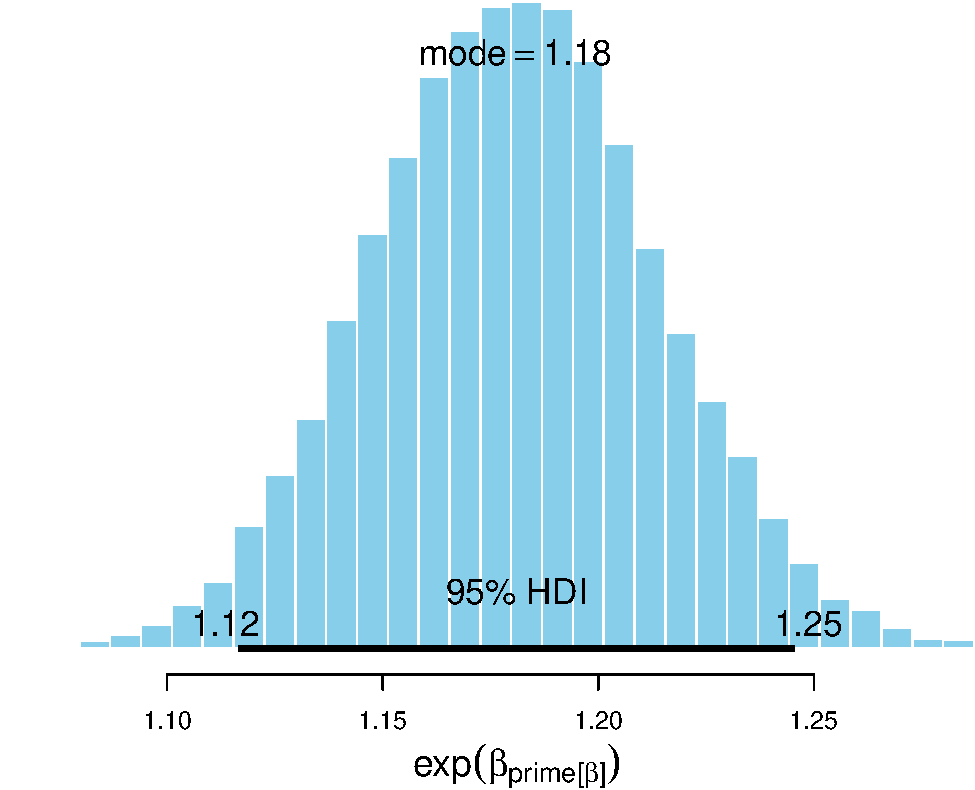
\includegraphics[width=0.5\linewidth]{supplementary_materials_files/figure-latex/posterior-bias-prime-1} 

}

\caption{Posterior distribution of the odds ratio between LSF and HSF primes on the starting point.}\label{fig:posterior-bias-prime}
\end{figure}

\newpage

\hypertarget{non-decision-time}{%
\subsubsection{Non-decision time}\label{non-decision-time}}

Recall that the non-decision time parameter can be interpreted as a measure of the time used by non-decisional processes such as stimulus encoding or motor response, and that the linear model for this parameter is on the log scale (i.e., we used a log link function): \(\log(\tau_{i}) = \beta_{0} + \beta_{1} \cdot \text{Group}_{i}\).

\begin{figure}[!htb]

{\centering 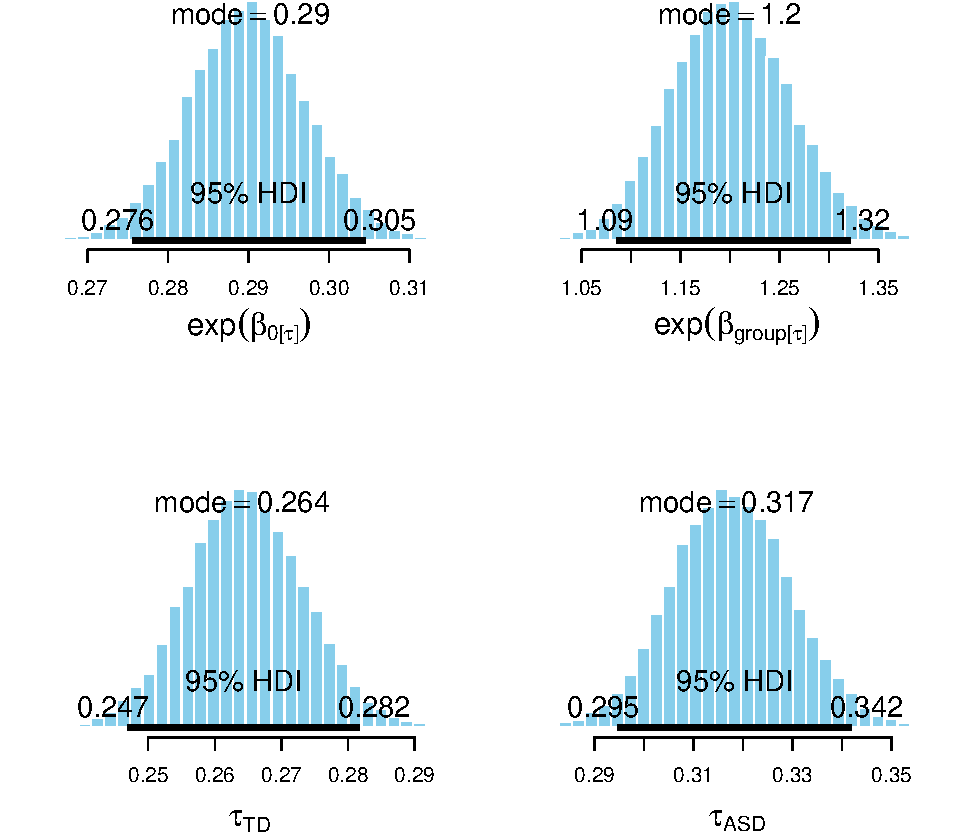
\includegraphics[width=0.75\linewidth]{supplementary_materials_files/figure-latex/posterior-ndt-1} 

}

\caption{Posterior distribution of the intercept and the slope for Group for the non-decision time. The upper two distributions are the distributions of the intercept and the slope (on the linear scale). The lower two plots are the posterior distributions of the non-decision time in the TD and ASD groups, respectively (on the linear scale).}\label{fig:posterior-ndt}
\end{figure}

Therefore, we have to apply the inverse link function (i.e., \(\exp(\cdot)\)) to the parameter to be able to interpret it. Taking \(\exp(\beta_{1})\) gives the proportional change in the value of the non-decision time parameter when we go from the TD group to the ASD group. In our case, \(\exp(\beta_{1}) \approx 1.24\) which means that going from TD to ASD leads to an increase of approximately 24 \% of the non-decision time parameter value. In other words, non-decisional processes seem to take longer in the ASD group than in the TD group.

\newpage

\hypertarget{evaluating-the-model}{%
\subsection{Evaluating the model}\label{evaluating-the-model}}

In Figure \ref{fig:ppc}, we depict the distribution of the raw data along with the distribution of ten simulated datasets.

\begin{Shaded}
\begin{Highlighting}[]
\KeywordTok{pp_check}\NormalTok{(varying_effects_prime, }\DataTypeTok{nsamples =} \DecValTok{10}\NormalTok{) }\OperatorTok{+}
\StringTok{  }\KeywordTok{theme_bw}\NormalTok{(}\DataTypeTok{base_size =} \DecValTok{12}\NormalTok{) }\OperatorTok{+}
\StringTok{  }\KeywordTok{labs}\NormalTok{(}\DataTypeTok{x =} \StringTok{"Response time (in seconds)"}\NormalTok{, }\DataTypeTok{y =} \StringTok{"Density"}\NormalTok{)}
\end{Highlighting}
\end{Shaded}

\begin{figure}[!htb]

{\centering 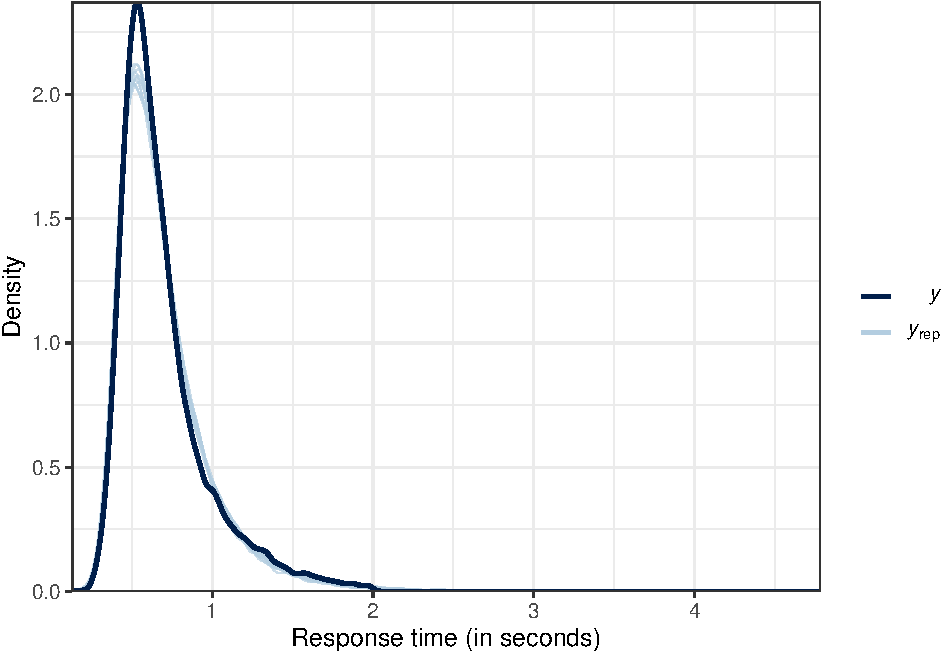
\includegraphics[width=0.75\linewidth]{supplementary_materials_files/figure-latex/ppc-1} 

}

\caption{Posterior predictive checking. The dark blue line represents the distribution of raw data whereas light blue lines represent data simulated from the posterior distribution.}\label{fig:ppc}
\end{figure}

As can be seen from Figure \ref{fig:ppc}, the model seems pretty good at simulating data that looks like the observed data. From this predictive/sampling distribution (i.e., the distribution of simulated data sets), so-called \enquote{Bayesian \emph{p}-values} can be computed to quantify the compatibility between the observed data and the proposed model.

\newpage

\hypertarget{hypothesis-testing}{%
\subsection{Hypothesis testing}\label{hypothesis-testing}}

We can test any arbitrary hypothesis using the \texttt{brms::hypothesis()} method, which is computing a Bayes factor via the Savage-Dickey method (Wagenmakers, Lodewyckx, Kuriyal, \& Grasman, \protect\hyperlink{ref-wagenmakers_bayesian_2010}{2010}), which consists in comparing the posterior probability density to the prior probability density for some hypothesised value for the parameter of interest (e.g., \(\theta = 0\)).

\begin{Shaded}
\begin{Highlighting}[]
\CommentTok{# Plotting the Savage-Dickey Bayes factor}
\CommentTok{# testing whether the interaction Group * Congruency is equal to 0}
\NormalTok{hyp <-}\StringTok{ }\KeywordTok{hypothesis}\NormalTok{(varying_effects_prime, }\StringTok{"GroupC:CongC = 0"}\NormalTok{)}
\CommentTok{# prints the output}
\KeywordTok{print}\NormalTok{(hyp)}
\end{Highlighting}
\end{Shaded}

\begin{verbatim}
## Hypothesis Tests for class b:
##           Hypothesis Estimate Est.Error CI.Lower CI.Upper Evid.Ratio Post.Prob
## 1 (GroupC:CongC) = 0     -0.1      0.05     -0.2        0       3.16      0.76
##   Star
## 1     
## ---
## 'CI': 90%-CI for one-sided and 95%-CI for two-sided hypotheses.
## '*': For one-sided hypotheses, the posterior probability exceeds 95%;
## for two-sided hypotheses, the value tested against lies outside the 95%-CI.
## Posterior probabilities of point hypotheses assume equal prior probabilities.
\end{verbatim}

\begin{Shaded}
\begin{Highlighting}[]
\CommentTok{# plotting it}
\KeywordTok{data.frame}\NormalTok{(}\DataTypeTok{posterior =}\NormalTok{ hyp}\OperatorTok{$}\NormalTok{samples}\OperatorTok{$}\NormalTok{H1, }\DataTypeTok{prior =}\NormalTok{ hyp}\OperatorTok{$}\NormalTok{prior_samples}\OperatorTok{$}\NormalTok{H1) }\OperatorTok
\StringTok{  }\KeywordTok{gather}\NormalTok{(type, value) }\OperatorTok
\StringTok{  }\KeywordTok{ggplot}\NormalTok{(}\KeywordTok{aes}\NormalTok{(}\DataTypeTok{x =}\NormalTok{ value, }\DataTypeTok{fill =}\NormalTok{ type) ) }\OperatorTok{+}
\StringTok{  }\KeywordTok{geom_vline}\NormalTok{(}\DataTypeTok{xintercept =} \DecValTok{0}\NormalTok{, }\DataTypeTok{linetype =} \DecValTok{3}\NormalTok{, }\DataTypeTok{alpha =} \DecValTok{1}\NormalTok{) }\OperatorTok{+}
\StringTok{  }\KeywordTok{geom_area}\NormalTok{(}\DataTypeTok{stat =} \StringTok{"density"}\NormalTok{, }\DataTypeTok{alpha =} \FloatTok{0.8}\NormalTok{, }\DataTypeTok{position =} \StringTok{"identity"}\NormalTok{) }\OperatorTok{+}
\StringTok{  }\KeywordTok{theme_bw}\NormalTok{(}\DataTypeTok{base_size =} \DecValTok{12}\NormalTok{) }\OperatorTok{+}
\StringTok{  }\KeywordTok{labs}\NormalTok{(}\DataTypeTok{x =} \KeywordTok{expression}\NormalTok{(beta[group}\OperatorTok{:}\NormalTok{congruency]), }\DataTypeTok{y =} \StringTok{"Probability density"}\NormalTok{) }\OperatorTok{+}
\StringTok{  }\KeywordTok{scale_fill_brewer}\NormalTok{(}\DataTypeTok{palette =} \StringTok{"Dark2"}\NormalTok{, }\DataTypeTok{direction =} \DecValTok{-1}\NormalTok{) }\OperatorTok{+}
\StringTok{  }\KeywordTok{theme}\NormalTok{(}\DataTypeTok{legend.title =} \KeywordTok{element_blank}\NormalTok{() ) }\OperatorTok{+}
\StringTok{  }\KeywordTok{coord_cartesian}\NormalTok{(}\DataTypeTok{xlim =} \KeywordTok{c}\NormalTok{(}\OperatorTok{-}\DecValTok{2}\NormalTok{, }\DecValTok{2}\NormalTok{) )}
\end{Highlighting}
\end{Shaded}

\begin{figure}[!htb]

{\centering 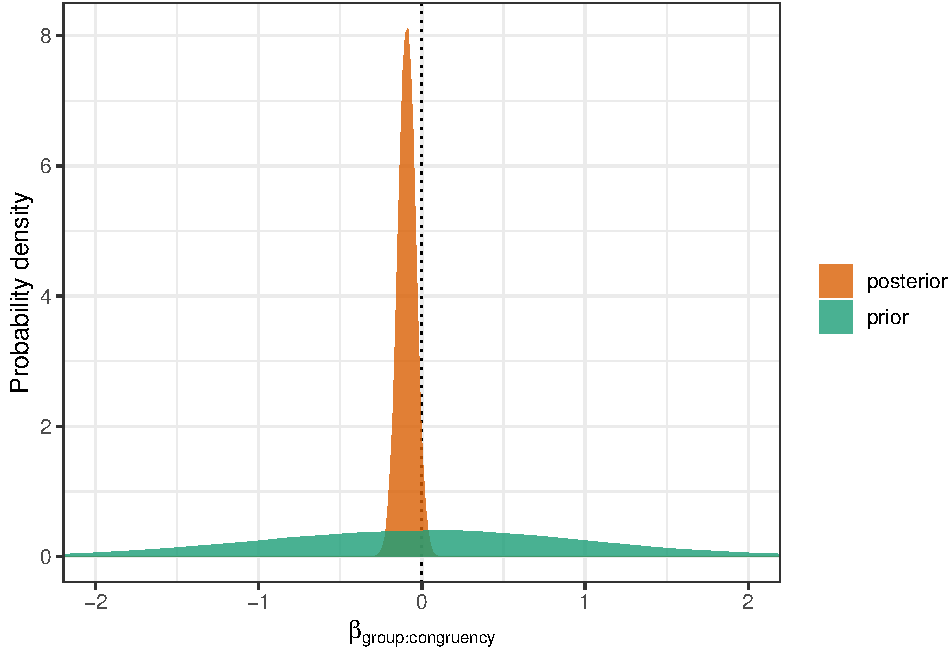
\includegraphics[width=0.75\linewidth]{supplementary_materials_files/figure-latex/hypothesis1-1} 

}

\caption{Hypothesis testing via the Savage-Dickey method. The resulting Bayes factor (BF) is the ratio of the height (i.e., the density probability) of the posterior versus prior distribution at some value of interest for the parameter (here it is 0).}\label{fig:hypothesis1}
\end{figure}

The resulting Bayes factor (called \enquote{Evid. Ratio} in the output) may be interpreted as follows: the observed data is 4.09 more likely under the hypothesis of null effect than under the hypothesis of a non-null effect. Alternatively, the BF can be interpreted as an \emph{updating factor}, indicating by \enquote{how much} we should update our \emph{prior odds} (the ratio of the a priori probability of \(H_{0}\) versus \(H_{1}\)) to convert them into \emph{posterior odds} (the ratio of the a posteriori probability of \(H_{0}\) versus \(H_{1}\)). Note however that the BF is highly dependent on the prior put on the parameter. In this example, we see that despite the fact that the posterior distribution is \enquote{less centered} on 0 than the prior distribution, because of the vagueness of the prior distribution, the posterior distribution still allocates more probability density to 0 than the prior distribution does.

\begin{table}[htb]

\begin{center}
\begin{threeparttable}

\caption{\label{tab:summary}Estimates and BFs for the slopes from the hierarchical DDM.}

\begin{tabular}{ccccccc}
\toprule
Term & \multicolumn{1}{c}{Estimate} & \multicolumn{1}{c}{SE} & \multicolumn{1}{c}{Lower} & \multicolumn{1}{c}{Upper} & \multicolumn{1}{c}{Rhat} & \multicolumn{1}{c}{BF01}\\
\midrule
GroupC & -0.012 & 0.204 & -0.416 & 0.383 & 1.002 & 4.872\\
CongC & 0.325 & 0.027 & 0.273 & 0.378 & 1.000 & 5.533*10\textasciicircum{}-17\\
PrimeC & -0.113 & 0.042 & -0.195 & -0.032 & 1.000 & 0.516\\
GroupC:CongC & -0.099 & 0.053 & -0.201 & 0.003 & 1.000 & 3.162\\
GroupC:PrimeC & 0.048 & 0.084 & -0.116 & 0.213 & 1.000 & 9.958\\
CongC:PrimeC & 0.063 & 0.053 & -0.040 & 0.167 & 1.000 & 8.975\\
GroupC:CongC:PrimeC & -0.022 & 0.106 & -0.233 & 0.187 & 1.001 & 9.153\\
bs\_GroupC & 0.079 & 0.060 & -0.039 & 0.196 & 1.001 & 6.715\\
ndt\_GroupC & 0.182 & 0.051 & 0.084 & 0.282 & 1.001 & 0.011\\
bias\_GroupC & 0.012 & 0.081 & -0.147 & 0.169 & 1.001 & 12.058\\
bias\_PrimeC & 0.161 & 0.027 & 0.109 & 0.213 & 1.000 & 1.618*10\textasciicircum{}-17\\
bias\_GroupC:PrimeC & -0.022 & 0.054 & -0.127 & 0.084 & 1.000 & 17.235\\
\bottomrule
\addlinespace
\end{tabular}

\begin{tablenotes}[para]
\normalsize{\textit{Note.} For each slope (for each line), the first two columns represent the estimated
    most probable value and its standard error (SE). The 'Lower' and 'Upper' columns
    contain the lower and upper bounds of the 95\% CrI, whereas the 'Rhat' column reports
    the Gelman-Rubin statistic. The last column reports the Bayes factor in favour of the
    null hypothesis (BF01).}
\end{tablenotes}

\end{threeparttable}
\end{center}

\end{table}

Finally, Table \ref{tab:summary} reports the estimates and associated credible intervals and \(\text{BF01}\)s for all slopes in the hierarchical DDM. To sum up our results, these estimates suggest that \texttt{Cong} increasew the drift rate, while \texttt{Prime} seems to decrease it, which means that congruent (vs.~incongruent) and LSF (vs.~HSF) stimuli increase the ease of processing of the stimulus. The positive effect of \texttt{Group} on the non-decision time parameter suggests non-decision related processes (such as the stimulus processing or motor processes) are different according to the group (i.e., they take longer in the ASD group than in the TD group). Finally, the effect of \texttt{Prime} on the starting point suggests that HSF (vs.~LSF) primes were associated with an a priori \enquote{bias} towards accurate responses.

\hypertarget{acknowledgments}{%
\section{Acknowledgments}\label{acknowledgments}}

Most of the computations presented in this paper were performed using the GRICAD infrastructure (\url{https://gricad.univ-grenoble-alpes.fr}), which is partly supported by the \href{mailto:Equip@Meso}{\nolinkurl{Equip@Meso}} project (reference ANR-10-EQPX-29-01) of the programme Investissements d'Avenir supervised by the Agence Nationale pour la Recherche.

\newpage

\hypertarget{session-information}{%
\section{Session information}\label{session-information}}

\begin{Shaded}
\begin{Highlighting}[]
\KeywordTok{sessionInfo}\NormalTok{()}
\end{Highlighting}
\end{Shaded}

\begin{verbatim}
## R version 4.0.3 (2020-10-10)
## Platform: x86_64-apple-darwin17.0 (64-bit)
## Running under: macOS Big Sur 10.16
## 
## Matrix products: default
## BLAS:   /Library/Frameworks/R.framework/Versions/4.0/Resources/lib/libRblas.dylib
## LAPACK: /Library/Frameworks/R.framework/Versions/4.0/Resources/lib/libRlapack.dylib
## 
## locale:
## [1] C/en_US.UTF-8/C/C/C/C
## 
## attached base packages:
## [1] parallel  stats     graphics  grDevices utils     datasets  methods  
## [8] base     
## 
## other attached packages:
##  [1] emmeans_1.5.4          BayesFactor_0.9.12-4.2 Matrix_1.3-2          
##  [4] coda_0.19-4            flextable_0.6.3        ggpubr_0.4.0          
##  [7] kableExtra_1.3.1       qwraps2_0.5.0          car_3.0-10            
## [10] carData_3.0-4          reshape2_1.4.4         lattice_0.20-41       
## [13] plyr_1.8.6             here_1.0.1             ggrepel_0.9.1         
## [16] patchwork_1.1.1        BEST_0.5.2             HDInterval_0.2.2      
## [19] brms_2.14.4            Rcpp_1.0.6             glue_1.4.2            
## [22] knitr_1.31             papaja_0.1.0.9997      tinylabels_0.2.0      
## [25] forcats_0.5.1          stringr_1.4.0          dplyr_1.0.4           
## [28] purrr_0.3.4            readr_1.4.0            tidyr_1.1.2           
## [31] tibble_3.0.6           ggplot2_3.3.3          tidyverse_1.3.0       
## 
## loaded via a namespace (and not attached):
##   [1] uuid_0.1-4           readxl_1.3.1         backports_1.2.1     
##   [4] systemfonts_1.0.0    igraph_1.2.6         splines_4.0.3       
##   [7] crosstalk_1.1.1      rstantools_2.1.1     inline_0.3.17       
##  [10] digest_0.6.27        htmltools_0.5.1.1    rsconnect_0.8.16    
##  [13] magrittr_2.0.1       openxlsx_4.2.3       modelr_0.1.8        
##  [16] RcppParallel_5.0.2   matrixStats_0.58.0   officer_0.3.16      
##  [19] xts_0.12.1           prettyunits_1.1.1    colorspace_2.0-0    
##  [22] rvest_0.3.6          haven_2.3.1          xfun_0.20           
##  [25] callr_3.5.1          crayon_1.4.0         jsonlite_1.7.2      
##  [28] lme4_1.1-26          zoo_1.8-8            gtable_0.3.0        
##  [31] MatrixModels_0.4-1   webshot_0.5.2        V8_3.4.0            
##  [34] pkgbuild_1.2.0       rstan_2.21.2         abind_1.4-5         
##  [37] scales_1.1.1         mvtnorm_1.1-1        DBI_1.1.1           
##  [40] rstatix_0.6.0        miniUI_0.1.1.1       viridisLite_0.3.0   
##  [43] xtable_1.8-4         foreign_0.8-81       stats4_4.0.3        
##  [46] StanHeaders_2.21.0-7 DT_0.17              htmlwidgets_1.5.3   
##  [49] httr_1.4.2           threejs_0.3.3        ellipsis_0.3.1      
##  [52] farver_2.0.3         pkgconfig_2.0.3      loo_2.4.1           
##  [55] dbplyr_2.1.0         labeling_0.4.2       tidyselect_1.1.0    
##  [58] rlang_0.4.10         later_1.1.0.1        munsell_0.5.0       
##  [61] cellranger_1.1.0     tools_4.0.3          cli_2.3.0           
##  [64] generics_0.1.0       broom_0.7.4.9000     ggridges_0.5.3      
##  [67] evaluate_0.14        fastmap_1.1.0        yaml_2.2.1          
##  [70] processx_3.4.5       fs_1.5.0             zip_2.1.1           
##  [73] pbapply_1.4-3        nlme_3.1-152         mime_0.9            
##  [76] projpred_2.0.2       xml2_1.3.2           compiler_4.0.3      
##  [79] bayesplot_1.8.0      shinythemes_1.2.0    rstudioapi_0.13     
##  [82] gamm4_0.2-6          curl_4.3             ggsignif_0.6.0      
##  [85] reprex_1.0.0         statmod_1.4.35       stringi_1.5.3       
##  [88] ps_1.5.0             Brobdingnag_1.2-6    gdtools_0.2.3       
##  [91] nloptr_1.2.2.2       markdown_1.1         shinyjs_2.0.0       
##  [94] vctrs_0.3.6          pillar_1.4.7         lifecycle_0.2.0     
##  [97] bridgesampling_1.0-0 estimability_1.3     data.table_1.13.6   
## [100] httpuv_1.5.5         R6_2.5.0             bookdown_0.21       
## [103] promises_1.1.1       rio_0.5.16           gridExtra_2.3       
## [106] rjags_4-10           codetools_0.2-18     boot_1.3-26         
## [109] colourpicker_1.1.0   MASS_7.3-53          gtools_3.8.2        
## [112] assertthat_0.2.1     rprojroot_2.0.2      withr_2.4.1         
## [115] shinystan_2.5.0      mgcv_1.8-33          hms_1.0.0           
## [118] grid_4.0.3           minqa_1.2.4          rmarkdown_2.6       
## [121] shiny_1.6.0          lubridate_1.7.9.2    base64enc_0.1-3     
## [124] dygraphs_1.1.1.6
\end{verbatim}

\newpage

\hypertarget{references}{%
\section*{References}\label{references}}
\addcontentsline{toc}{section}{References}

\hypertarget{refs}{}
\leavevmode\hypertarget{ref-R-papaja}{}%
Aust, F., \& Barth, M. (2020). \emph{papaja: Create APA manuscripts with R Markdown}. Retrieved from \url{https://github.com/crsh/papaja}

\leavevmode\hypertarget{ref-barr_random_2013-1}{}%
Barr, D. J., Levy, R., Scheepers, C., \& Tily, H. J. (2013). Random effects structure for confirmatory hypothesis testing: Keep it maximal. \emph{Journal of Memory and Language}, \emph{68}(3), 255--278. \url{https://doi.org/10.1016/j.jml.2012.11.001}

\leavevmode\hypertarget{ref-R-brms_a}{}%
Bürkner, P.-C. (2017). brms: An R package for Bayesian multilevel models using Stan. \emph{Journal of Statistical Software}, \emph{80}(1), 1--28. \url{https://doi.org/10.18637/jss.v080.i01}

\leavevmode\hypertarget{ref-forstmann_sequential_2016}{}%
Forstmann, B. U., Ratcliff, R., \& Wagenmakers, E.-J. (2016). Sequential Sampling Models in Cognitive Neuroscience: Advantages, Applications, and Extensions. \emph{Annual Review of Psychology}, \emph{67}, 641--666. \url{https://doi.org/10.1146/annurev-psych-122414-033645}

\leavevmode\hypertarget{ref-gabry_visualization_2019}{}%
Gabry, J., Simpson, D., Vehtari, A., Betancourt, M., \& Gelman, A. (2019). Visualization in Bayesian workflow. \emph{Journal of the Royal Statistical Society: Series A (Statistics in Society)}, \emph{182}(2), 389--402. \url{https://doi.org/10.1111/rssa.12378}

\leavevmode\hypertarget{ref-ratcliff_theory_1978}{}%
Ratcliff, R. (1978). A theory of memory retrieval. \emph{Psychological Review}, \emph{85}(2), 59--108. \url{https://doi.org/10.1037/0033-295X.85.2.59}

\leavevmode\hypertarget{ref-ratcliff_diffusion_2008}{}%
Ratcliff, R., \& McKoon, G. (2008). The diffusion decision model: Theory and data for two-choice decision tasks. \emph{Neural Computation}, \emph{20}(4), 873--922. \url{https://doi.org/10.1162/neco.2008.12-06-420}

\leavevmode\hypertarget{ref-R-base}{}%
R Core Team. (2019). \emph{R: A language and environment for statistical computing}. Vienna, Austria: R Foundation for Statistical Computing. Retrieved from \url{https://www.R-project.org/}

\leavevmode\hypertarget{ref-singmann_diffusionux2fwiener_2017}{}%
Singmann, H. (2017). Diffusion/Wiener Model Analysis with brms -- Part I: Introduction and Estimation. Retrieved from \url{http://singmann.org/wiener-model-analysis-with-brms-part-i/}

\leavevmode\hypertarget{ref-vandekerckhove_crossed_2010}{}%
Vandekerckhove, J., Verheyen, S., \& Tuerlinckx, F. (2010). A crossed random effects diffusion model for speeded semantic categorization decisions. \emph{Acta Psychologica}, \emph{133}(3), 269--282. \url{https://doi.org/10.1016/j.actpsy.2009.10.009}

\leavevmode\hypertarget{ref-vinding_volition_2018}{}%
Vinding, M., Lindeløv, J. K., Xiao, Y., Chan, R. C. K., \& Sørensen, T. A. (2018). \emph{Volition in Prospective Memory: Evidence against differences in recalling free and fixed delayed intentions}. \url{https://doi.org/10.31234/osf.io/hsrbt}

\leavevmode\hypertarget{ref-wabersich_rwiener_2014}{}%
Wabersich, D., \& Vandekerckhove, J. (2014). The RWiener Package: An R Package Providing Distribution Functions for the Wiener Diffusion Model. \emph{The R Journal}, \emph{6}(1), 49--56. Retrieved from \url{https://journal.r-project.org/archive/2014/RJ-2014-005/index.html}

\leavevmode\hypertarget{ref-wagenmakers_methodological_2009-1}{}%
Wagenmakers, E.-J. (2009). Methodological and empirical developments for the Ratcliff diffusion model of response times and accuracy. \emph{European Journal of Cognitive Psychology}, \emph{21}(5), 641--671. \url{https://doi.org/10.1080/09541440802205067}

\leavevmode\hypertarget{ref-wagenmakers_bayesian_2010}{}%
Wagenmakers, E.-J., Lodewyckx, T., Kuriyal, H., \& Grasman, R. (2010). Bayesian hypothesis testing for psychologists: A tutorial on the Savage--Dickey method. \emph{Cognitive Psychology}, \emph{60}(3), 158--189. \url{https://doi.org/10.1016/j.cogpsych.2009.12.001}

\leavevmode\hypertarget{ref-wagenmakers_ez-diffusion_2007}{}%
Wagenmakers, E.-J., Van Der Maas, H. L. J., \& Grasman, R. P. P. P. (2007). An EZ-diffusion model for response time and accuracy. \emph{Psychonomic Bulletin \& Review}, \emph{14}(1), 3--22. \url{https://doi.org/10.3758/BF03194023}

\leavevmode\hypertarget{ref-R-tidyverse}{}%
Wickham, H., Averick, M., Bryan, J., Chang, W., McGowan, L. D., François, R., \ldots{} Yutani, H. (2019). Welcome to the tidyverse. \emph{Journal of Open Source Software}, \emph{4}(43), 1686. \url{https://doi.org/10.21105/joss.01686}

\leavevmode\hypertarget{ref-R-knitr}{}%
Xie, Y. (2015). \emph{Dynamic documents with R and knitr} (2nd ed.). Boca Raton, Florida: Chapman; Hall/CRC. Retrieved from \url{https://yihui.org/knitr/}


\end{document}
